\section{Extremum estimators}\label{sec:A-extremum}

Almost every estimator in this book maximizes or minimizes a criterion function. Least squares minimizes a sum of squared
residuals. Maximum likelihood maximizes a log-likelihood. The BLP estimator minimizes a quadratic form in sample moments.
Simulated versions replace an intractable integral inside the criterion by an average over random draws. It pays to
prove consistency and asymptotic normality once, for the whole class, and then to read off each special case. This
section does that, following \citet{NeweyMcFadden1994}. As in the rest of the appendix, $\theta$ is a generic parameter
vector, here of dimension $K$, and the data $w_1, \dots, w_n$ are independent and identically distributed unless stated
otherwise. The convergence notation is the one set out in the introduction to this appendix.

\begin{definition}[Extremum estimator]\label{def:A-extremum}
Let $\Theta \subset \R^K$ be a parameter space and $Q_n(\theta)$ a criterion function that depends on the data. An
\emph{extremum estimator} is any $\hat\theta \in \Theta$ with
\begin{equation}\label{eq:A-extremum}
  Q_n(\hat\theta) \ge \sup_{\theta \in \Theta} Q_n(\theta) - o_p(1).
\end{equation}
The \emph{limit criterion} is a nonrandom function $Q_0(\theta)$ to which $Q_n(\theta)$ converges in probability.
\end{definition}

The $o_p(1)$ slack in \eqref{eq:A-extremum} allows for numerical optimization that stops close to, but not exactly at, the
supremum. This slack is enough for consistency. Asymptotic normality needs a tighter optimization tolerance, condition (v)
of \cref{thm:A-asy-normal}. The leading examples are the following.
\begin{enumerate}
  \item \emph{Nonlinear least squares} sets $Q_n(\theta) = -\frac{1}{n}\sum_{i=1}^n\{y_i - m(x_i;\theta)\}^2$, with limit
  $Q_0(\theta) = -\E[\{y_i - m(x_i;\theta)\}^2]$. Ordinary least squares is the case $m(x;\theta) = x^\T\theta$.
  \item \emph{Maximum likelihood} sets $Q_n(\theta) = \frac{1}{n}\sum_{i=1}^n\ln f(y_i \mid x_i;\theta)$, with limit
  $Q_0(\theta) = \E[\ln f(y_i \mid x_i;\theta)]$ (\cref{sec:A-mle}).
  \item The \emph{generalized method of moments} sets
  $Q_n(\theta) = -\bar g_n(\theta)^\T W_n\bar g_n(\theta)$, with limit
  $Q_0(\theta) = -\E[g(w_i;\theta)]^\T W\E[g(w_i;\theta)]$ (\cref{sec:A-gmm}). Here
  $\bar g_n(\theta) = \frac{1}{n}\sum_i g(w_i;\theta)$, and $W_n$ is a weighting matrix.
  \item \emph{Simulated estimators} use the same criteria with an expectation inside $g$ or $f$ replaced by a
  simulation average (\cref{sec:A-simulation}).
\end{enumerate}
The first two are \emph{M-estimators}, because $Q_n$ is a sample average of a function of one observation. GMM is a
\emph{minimum distance} estimator, because $Q_n$ is a quadratic form in sample averages. The general theorems below cover
both.

\subsection{Consistency}\label{sec:A-ext-consistency}

Consistency rests on two ideas. The limit criterion must have a unique maximum at the true value. The sample criterion
must be close to the limit criterion everywhere on the parameter space, not only at each point separately.

\begin{theorem}[Consistency of extremum estimators]\label{thm:A-consistency}
Suppose that (i) $Q_0(\theta)$ is uniquely maximized at $\theta_0$ (identification), (ii) $\Theta$ is compact, (iii)
$Q_0(\theta)$ is continuous, and (iv) $\sup_{\theta \in \Theta}\lvert Q_n(\theta) - Q_0(\theta)\rvert \xrightarrow{p} 0$
(uniform convergence). Then any extremum estimator satisfies $\hat\theta \xrightarrow{p} \theta_0$.
\end{theorem}

\begin{proof}
Fix $\epsilon > 0$. Three events occur w.p.a.1. By \eqref{eq:A-extremum},
$Q_n(\hat\theta) > Q_n(\theta_0) - \frac{\epsilon}{3}$. By uniform convergence,
$Q_0(\hat\theta) > Q_n(\hat\theta) - \frac{\epsilon}{3}$, since $\hat\theta \in \Theta$. Again by uniform convergence,
$Q_n(\theta_0) > Q_0(\theta_0) - \frac{\epsilon}{3}$. Chaining the three inequalities gives, w.p.a.1,
\begin{equation}\label{eq:A-consistency-chain}
  Q_0(\hat\theta) > Q_n(\hat\theta) - \frac{\epsilon}{3} > Q_n(\theta_0) - \frac{2\epsilon}{3} > Q_0(\theta_0) - \epsilon.
\end{equation}
Now let $\mathcal{N}$ be any open set that contains $\theta_0$. The set $\Theta \cap \mathcal{N}^c$ is closed and bounded,
hence compact. Since $Q_0$ is continuous, it attains its supremum on this set at some $\theta^*$. Identification gives
$Q_0(\theta^*) < Q_0(\theta_0)$. Choose $\epsilon = Q_0(\theta_0) - Q_0(\theta^*) > 0$. Then
\eqref{eq:A-consistency-chain} says that, w.p.a.1,
\begin{equation*}
  Q_0(\hat\theta) > Q_0(\theta^*) = \sup_{\theta \in \Theta \cap \mathcal{N}^c}Q_0(\theta).
\end{equation*}
So $\hat\theta \notin \Theta \cap \mathcal{N}^c$, that is, $\hat\theta \in \mathcal{N}$, w.p.a.1. Because $\mathcal{N}$ was
arbitrary, $\hat\theta \xrightarrow{p} \theta_0$.
\end{proof}

\Cref{fig:A-extremum} draws the argument. Uniform convergence traps $Q_n$ in a band of half-width $\epsilon$ around
$Q_0$. The maximizer of $Q_n$ must then achieve a value of $Q_0$ within $2\epsilon$ of the maximum, and identification
confines such points to a neighborhood of $\theta_0$ that shrinks with $\epsilon$.

\begin{figure}[htbp]
\centering
\begin{tikzpicture}
\begin{axis}[
  width=0.82\textwidth, height=6.2cm,
  xmin=0.2, xmax=3.8, ymin=0, ymax=2.75,
  axis lines=left, xlabel={$\theta$}, ylabel={criterion},
  xtick={0.8168, 2, 2.3087, 3.1832},
  xticklabels={$\theta_0 - r_\epsilon$, $\theta_0$, $\hat\theta$, $\theta_0 + r_\epsilon$},
  ytick={1.3, 2}, yticklabels={$Q_0(\theta_0) - 2\epsilon$, $Q_0(\theta_0)$},
  every tick label/.append style={font=\footnotesize},
  samples=200, domain=0.3:3.7, clip=false]
  \addplot[name path=up, draw=none, forget plot] {2 - 0.5*(x-2)^2 + 0.35};
  \addplot[name path=dn, draw=none, forget plot] {2 - 0.5*(x-2)^2 - 0.35};
  \addplot[blue!12, forget plot] fill between[of=up and dn];
  \addplot[blue!60!black, dashed, thin, forget plot] {2 - 0.5*(x-2)^2 + 0.35};
  \addplot[blue!60!black, dashed, thin, forget plot] {2 - 0.5*(x-2)^2 - 0.35};
  \addplot[black, very thick] {2 - 0.5*(x-2)^2};
  \addplot[orange!85!black, thick] {2 - 0.5*(x-2)^2 + 0.22*sin(deg(2.6*x+0.5)) + 0.1*sin(deg(6.3*x))};
  \draw[gray, densely dotted] (axis cs:0.2,1.3) -- (axis cs:3.8,1.3);
  \draw[gray, densely dotted] (axis cs:0.2,2) -- (axis cs:2,2);
  \draw[gray, densely dotted] (axis cs:0.8168,0) -- (axis cs:0.8168,1.3);
  \draw[gray, densely dotted] (axis cs:3.1832,0) -- (axis cs:3.1832,1.3);
  \draw[gray, densely dotted] (axis cs:2,0) -- (axis cs:2,2);
  \draw[orange!85!black, densely dotted] (axis cs:2.3087,0) -- (axis cs:2.3087,2.092);
  \fill[orange!85!black] (axis cs:2.3087,2.092) circle (1.6pt);
  \draw[very thick, gray!70] (axis cs:0.8168,0.06) -- (axis cs:3.1832,0.06);
  \draw[black, thin] (axis cs:3.0,1.5) -- (axis cs:3.45,2.05);
  \node[font=\footnotesize, anchor=south west] at (axis cs:3.42,2.03) {$Q_0(\theta)$};
  \draw[orange!85!black, thin] (axis cs:0.9,1.402) -- (axis cs:0.6,1.95);
  \node[font=\footnotesize, anchor=south, text=orange!85!black] at (axis cs:0.6,1.93) {$Q_n(\theta)$};
  \node[font=\footnotesize, anchor=south, text=blue!60!black] at (axis cs:2.2,2.4) {$Q_0(\theta) \pm \epsilon$};
\end{axis}
\end{tikzpicture}
\caption[The consistency argument for extremum estimators]{The consistency argument for extremum estimators. The thick
curve is the limit criterion $Q_0$, maximized only at $\theta_0$. Uniform convergence places the sample criterion $Q_n$
inside the shaded band $Q_0 \pm \epsilon$. The maximizer $\hat\theta$ of $Q_n$ then satisfies $Q_0(\hat\theta) > Q_0(\theta_0)
- 2\epsilon$, so it lies in the interval $[\theta_0 - r_\epsilon, \theta_0 + r_\epsilon]$ marked on the horizontal axis.
The curves are illustrative: $Q_0(\theta) = 2 - \frac{1}{2}(\theta - 2)^2$ and $\epsilon = 0.35$.}
\label{fig:A-extremum}
\end{figure}

Pointwise convergence of $Q_n(\theta)$ to $Q_0(\theta)$ at each $\theta$ is not enough. Take $\Theta = [0, 2]$ and
\begin{equation*}
  Q_n(\theta) = -\theta^2 + 2\max\left\{0,\ 1 - n\left\lvert\theta - 1 - \frac{1}{n}\right\rvert\right\}.
\end{equation*}
At each fixed $\theta$ the spike eventually moves away, so $Q_n(\theta) \to Q_0(\theta) = -\theta^2$, which is maximized at
$0$. Yet $Q_n(1 + \frac{1}{n}) = 2 - (1 + \frac{1}{n})^2$ is close to $1$, above $Q_n(0) = 0$. The maximizer converges to
$1$, not to $0$. Uniform convergence fails because $\sup_\theta\lvert Q_n - Q_0\rvert = 2$ for every $n$.

Uniform convergence is usually verified with a uniform law of large numbers. The next lemma is the version we use most
often. It is \citet[Lemma 2.4]{NeweyMcFadden1994}.

\begin{lemma}[Uniform law of large numbers]\label{lem:A-ulln}
Let $w_i$ be i.i.d., $\Theta$ compact, and $a(w, \theta)$ continuous in $\theta$ at each $\theta \in \Theta$ with
probability one. If $\E[\sup_{\theta \in \Theta}\lVert a(w_i, \theta)\rVert] < \infty$, then $\E[a(w_i, \theta)]$ is
continuous and
\begin{equation*}
  \sup_{\theta \in \Theta}\left\lVert\frac{1}{n}\sum_{i=1}^n a(w_i, \theta) - \E[a(w_i, \theta)]\right\rVert
  \xrightarrow{p} 0.
\end{equation*}
\end{lemma}

The integrable envelope $\sup_\theta\lVert a(w, \theta)\rVert$ is the \emph{dominance condition}. Continuity and compactness
let us cover $\Theta$ by finitely many small balls. On each ball the function moves little, and the ordinary law of large
numbers applies at the finitely many centers. For maximum likelihood we apply the lemma to $a = \ln f$. For GMM we apply
it to $a = g$ and then use the continuity of the quadratic form.

Compactness is a nuisance in practice, since few applied parameter spaces are bounded. For concave criteria it can be
dropped. This matters for the logit and multinomial logit likelihoods, which are globally concave
(\cref{prop:A-logit-concave}).

\begin{theorem}[Consistency with a concave criterion]\label{thm:A-concave}
Suppose that $\theta_0$ is an interior point of a convex set $\Theta$, $Q_n(\theta)$ is concave on $\Theta$ for each $n$,
$Q_n(\theta) \xrightarrow{p} Q_0(\theta)$ for each $\theta \in \Theta$, and $Q_0$ is uniquely maximized at $\theta_0$. Then
$\hat\theta$ exists w.p.a.1 and $\hat\theta \xrightarrow{p} \theta_0$.
\end{theorem}

The proof \citep[Theorem 2.7]{NeweyMcFadden1994} uses a fact from convex analysis. Pointwise convergence of concave
functions implies uniform convergence on compact subsets of the interior. Apply \cref{thm:A-consistency} on a small closed
ball around $\theta_0$. Concavity then rules out a maximizer outside the ball. A concave function that is higher at the
center of a ball than everywhere on its boundary is also higher at the center than anywhere outside the ball.

Identification, condition (i), is the substantive assumption. It says that the model and the data distribution single
out $\theta_0$. \Cref{sec:A-identification} discusses what it requires in IO models. Conditions (ii) to (iv) are
regularity conditions that hold in most smooth applications.

\subsection{Asymptotic normality}\label{sec:A-ext-normality}

Once $\hat\theta$ is consistent, a Taylor expansion of the first-order condition around $\theta_0$ delivers its limit
distribution.

\begin{theorem}[Asymptotic normality of extremum estimators]\label{thm:A-asy-normal}
Suppose the following conditions hold.
\begin{enumerate}[label=(\roman*)]
  \item $\hat\theta \xrightarrow{p} \theta_0$, and $\theta_0$ is in the interior of $\Theta$.
  \item $Q_n(\theta)$ is twice continuously differentiable on a neighborhood $\mathcal{N}$ of $\theta_0$.
  \item $\sqrt{n}\,\nabla_\theta Q_n(\theta_0) \xrightarrow{d} N(0, \Sigma)$.
  \item There is a matrix function $H(\theta)$, continuous at $\theta_0$, with $\sup_{\theta \in
  \mathcal{N}}\lVert\nabla_{\theta\theta}Q_n(\theta) - H(\theta)\rVert \xrightarrow{p} 0$ and $H = H(\theta_0)$ nonsingular.
  \item $\sqrt{n}\,\nabla_\theta Q_n(\hat\theta) \xrightarrow{p} 0$. An exact interior maximizer satisfies this with
  $\nabla_\theta Q_n(\hat\theta) = 0$.
\end{enumerate}
Then
\begin{equation}\label{eq:A-sandwich}
  \sqrt{n}(\hat\theta - \theta_0) \xrightarrow{d} N\big(0,\ H^{-1}\Sigma H^{-1}\big).
\end{equation}
\end{theorem}

\begin{proof}
Because $\hat\theta \xrightarrow{p} \theta_0$ and $\theta_0$ is interior, $\hat\theta$ lies in $\mathcal{N}$ and in the
interior of $\Theta$ w.p.a.1. Write $r_n = \nabla_\theta Q_n(\hat\theta)$ for the gradient at the estimate. By (v),
$\sqrt{n}\,r_n \xrightarrow{p} 0$. Apply the mean value theorem to each element of the gradient. For row $k$ there is a point
$\bar\theta^{(k)}$ on the segment between $\hat\theta$ and $\theta_0$ with
\begin{equation*}
  r_{n,k} = \frac{\partial Q_n(\theta_0)}{\partial\theta_k} + \frac{\partial^2 Q_n(\bar\theta^{(k)})}{\partial\theta_k\partial\theta^\T}
  (\hat\theta - \theta_0).
\end{equation*}
Stack the rows into the matrix $\bar H_n$, whose row $k$ is the $k$-th row of the Hessian evaluated at $\bar\theta^{(k)}$.
Then
\begin{equation*}
  r_n = \nabla_\theta Q_n(\theta_0) + \bar H_n(\hat\theta - \theta_0).
\end{equation*}
Each $\bar\theta^{(k)}$ converges in probability to $\theta_0$. By (iv) and the continuity of $H$ at $\theta_0$,
\begin{equation*}
  \lVert\bar H_n - H\rVert \le \sup_{\theta \in \mathcal{N}}\lVert\nabla_{\theta\theta}Q_n(\theta) - H(\theta)\rVert
  + \max_k\lVert H(\bar\theta^{(k)}) - H\rVert \xrightarrow{p} 0.
\end{equation*}
So $\bar H_n$ is invertible w.p.a.1, and
\begin{equation*}
  \sqrt{n}(\hat\theta - \theta_0) = -\bar H_n^{-1}\sqrt{n}\,\nabla_\theta Q_n(\theta_0) + \bar H_n^{-1}\sqrt{n}\,r_n.
\end{equation*}
The second term converges in probability to zero by (v). By (iii), Slutsky's theorem and the continuous mapping theorem, the
right side converges in distribution to $-H^{-1}Z$ with $Z \sim N(0, \Sigma)$. Its variance is $H^{-1}\Sigma H^{-1}$, because
$H$ is symmetric.
\end{proof}

Condition (v) cannot be dropped. Take $Y_i$ i.i.d.\ $N(0,1)$, $\theta_0 = 0$, $Q_n(\theta) = -\frac{1}{2}(\theta - \bar Y)^2$,
and an optimizer that stops at $\hat\theta = \bar Y + n^{-\frac{1}{4}}$. The criterion shortfall is
$\frac{1}{2}n^{-\frac{1}{2}} = o(1)$, so $\hat\theta$ is a consistent extremum estimator and (i)--(iv) hold. Yet
$\sqrt{n}\,\hat\theta = \sqrt{n}\,\bar Y + n^{\frac{1}{4}}$ diverges. An optimization error that vanishes more slowly than
the sampling error swamps it. Under local quadratic curvature, a criterion shortfall of order $o_p(n^{-1})$ is enough for (v).

The variance in \eqref{eq:A-sandwich} is a \emph{sandwich}. The outer pieces measure the curvature of the criterion, the
inner piece the noise in its slope at the truth. A consistent estimator replaces $H$ by $\nabla_{\theta\theta}Q_n(\hat\theta)$
and $\Sigma$ by an estimate of the variance of $\sqrt{n}\,\nabla_\theta Q_n(\theta_0)$. For an M-estimator with
$Q_n = \frac{1}{n}\sum_i q(w_i;\theta)$, that estimate is $\frac{1}{n}\sum_i\nabla_\theta q(w_i;\hat\theta)
\nabla_\theta q(w_i;\hat\theta)^\T$. With dependent data it becomes a clustered or HAC estimate (\cref{sec:A-cluster,sec:A-hac}).

The theorem fails in three situations that occur in IO. If $\theta_0$ lies on the boundary of $\Theta$, the first-order
condition need not hold. A variance component or a regime probability equal to zero is the usual case
(\cref{sec:A-mle-nonregular}). If $Q_n$ is not differentiable, the expansion must be replaced by an argument based on
stochastic equicontinuity. Simulated frequency estimators and some auction estimators are examples
\citep{PakesPollard1989}. If $H$ is singular, the rank condition for local identification fails. The parameter
$\theta_0$ may still be identified through higher-order terms, but the normal approximation breaks down and the rate of
convergence changes.

\subsection{Profile objectives}\label{sec:A-profile}

Many IO estimators split the parameters into a block that is easy to optimize given the rest and a block that is hard.
Optimizing out the easy block first leaves a \emph{profile} (or \emph{concentrated}) criterion in the hard block alone.

\begin{proposition}[Profile criteria]\label{prop:A-profile}
Partition $\theta = (\theta_1, \theta_2)$ with $\Theta = \Theta_1 \times \Theta_2$. Suppose that for each $\theta_2$ the
maximizer $\hat\theta_1(\theta_2) = \argmax_{\theta_1 \in \Theta_1}Q_n(\theta_1, \theta_2)$ exists and is unique. Define the
profile criterion $\tilde Q_n(\theta_2) = Q_n(\hat\theta_1(\theta_2), \theta_2)$.
\begin{enumerate}[label=(\alph*)]
  \item $(\hat\theta_1, \hat\theta_2)$ maximizes $Q_n$ jointly if and only if $\hat\theta_2$ maximizes $\tilde Q_n$ and
  $\hat\theta_1 = \hat\theta_1(\hat\theta_2)$.
  \item Suppose $Q_n$ is twice continuously differentiable and that, on a neighborhood of $\theta_2$, $\hat\theta_1(\cdot)$ is
  continuous with values in the interior of $\Theta_1$. If the Hessian block $H_{11} = \nabla_{\theta_1\theta_1}Q_n$ is
  nonsingular at $(\hat\theta_1(\theta_2), \theta_2)$, then
  \begin{equation}\label{eq:A-profile-derivs}
    \nabla_{\theta_2}\tilde Q_n(\theta_2) = \nabla_{\theta_2}Q_n\big(\hat\theta_1(\theta_2), \theta_2\big),
    \qquad
    \nabla_{\theta_2\theta_2}\tilde Q_n(\theta_2) = H_{22} - H_{21}H_{11}^{-1}H_{12},
  \end{equation}
  where the blocks of the Hessian of $Q_n$ are evaluated at $(\hat\theta_1(\theta_2), \theta_2)$.
\end{enumerate}
\end{proposition}

\begin{proof}
(a) For any $(\theta_1, \theta_2)$,
\begin{equation*}
  Q_n(\theta_1, \theta_2) \le Q_n(\hat\theta_1(\theta_2), \theta_2) = \tilde Q_n(\theta_2).
\end{equation*}
Hence $\sup_{\theta}Q_n(\theta) = \sup_{\theta_2}\tilde Q_n(\theta_2)$. If $\hat\theta_2$ maximizes $\tilde Q_n$, then
$(\hat\theta_1(\hat\theta_2), \hat\theta_2)$ attains this common supremum. Conversely, if $(\hat\theta_1, \hat\theta_2)$
maximizes $Q_n$, then $\tilde Q_n(\hat\theta_2) \ge Q_n(\hat\theta_1, \hat\theta_2) = \sup_{\theta_2}\tilde Q_n$, and
uniqueness of the inner maximizer gives $\hat\theta_1 = \hat\theta_1(\hat\theta_2)$.

(b) Because the inner maximizer is interior, the inner first-order condition
$\nabla_{\theta_1}Q_n(\hat\theta_1(\theta_2), \theta_2) = 0$ holds on the neighborhood. The implicit function theorem gives
a locally unique $C^1$ solution of this condition. By continuity $\hat\theta_1(\cdot)$ coincides with it, and
differentiating the condition gives
\begin{equation*}
  H_{11}\frac{\partial\hat\theta_1}{\partial\theta_2^\T} + H_{12} = 0
  \quad\Longrightarrow\quad
  \frac{\partial\hat\theta_1}{\partial\theta_2^\T} = -H_{11}^{-1}H_{12}.
\end{equation*}
By the chain rule,
\begin{equation*}
  \nabla_{\theta_2}\tilde Q_n = \left(\frac{\partial\hat\theta_1}{\partial\theta_2^\T}\right)^\T\nabla_{\theta_1}Q_n
  + \nabla_{\theta_2}Q_n = \nabla_{\theta_2}Q_n,
\end{equation*}
because the first term vanishes by the inner first-order condition. This is the envelope theorem. Differentiating once
more,
\begin{equation*}
  \nabla_{\theta_2\theta_2}\tilde Q_n = H_{21}\frac{\partial\hat\theta_1}{\partial\theta_2^\T} + H_{22}
  = H_{22} - H_{21}H_{11}^{-1}H_{12}. \qedhere
\end{equation*}
\end{proof}

Part (a) is what makes nested estimation legitimate. Part (b) says how to get standard errors. By the partitioned
inverse formula, $(H_{22} - H_{21}H_{11}^{-1}H_{12})^{-1}$ is the $(2,2)$ block of $H^{-1}$. For maximum likelihood, where
the asymptotic variance is $(-H)^{-1}$, the inverse Hessian of the profile log-likelihood therefore gives the correct
variance for $\hat\theta_2$. It already accounts for the estimation of $\theta_1$. For GMM the full sandwich is needed,
and \cref{sec:A-gmm-computation} gives the formula.

Three applications recur in this book. In the normal linear regression, the variance $\sigma^2$ can be profiled out. The
log-likelihood at $\hat\sigma^2(\beta) = \frac{1}{n}\sum_i(y_i - x_i^\T\beta)^2$ is $-\frac{n}{2}\ln\hat\sigma^2(\beta)$ plus a
constant. This is the form behind the Cox statistic of \cref{prop:06-bres-cox}. In the BLP estimator, the linear demand
parameters have a closed form given the nonlinear ones (\cref{prop:08-concentrate}). In supply-side estimation with many
fixed effects, the effects and the linear cost parameters can be concentrated out by least squares.
\citet[p.~1780]{MillerWeinberg2017} do this when they estimate the internalization and cost parameters of the beer
industry after the MillerCoors joint venture (\cref{ch:mergers}).

Profiling does not cure an \emph{incidental parameters} problem. Suppose $y_{it} = \mu_i + e_{it}$ with
$e_{it} \sim N(0, \sigma^2)$, $i = 1, \dots, N$ and $t = 1, \dots, T$, with $T$ fixed and $N \to \infty$. Profiling out each
$\mu_i$ gives $\hat\mu_i = \bar y_i$ and
\begin{equation*}
  \hat\sigma^2 = \frac{1}{NT}\sum_{i=1}^N\sum_{t=1}^T(y_{it} - \bar y_i)^2 \xrightarrow{p} \frac{T - 1}{T}\sigma^2.
\end{equation*}
The estimator is inconsistent \citep{NeymanScott1948}. The number of profiled parameters grows with the sample, so the
fixed-dimension assumptions of \cref{thm:A-consistency} fail. In linear models the bias has a known form, but in nonlinear
models with many fixed effects it contaminates every parameter.

\subsection{Numerical practice}\label{sec:A-numerical}

The theorems describe the global maximizer. A computer returns a point where an algorithm stopped. The gap between the
two is a frequent source of error in structural IO, and good practice narrows it.

Gradient methods iterate $\theta^{(m+1)} = \theta^{(m)} - \lambda_m A_m^{-1}\nabla_\theta Q_n(\theta^{(m)})$, where
$\lambda_m > 0$ is a step length and $A_m$ approximates the Hessian. Newton's method uses the Hessian itself and converges
quadratically near a maximum with a negative definite Hessian. Quasi-Newton methods such as BFGS build $A_m$ from
successive gradients. For maximum likelihood, the method of \citet{BerndtEtAl1974} (BHHH) replaces the Hessian by minus
the outer product of the scores. That matrix is negative semidefinite by construction. By the information equality of
\cref{sec:A-mle-score}, it is consistent for the Hessian at the truth. Derivative-free methods such as Nelder and Mead's simplex need only
function values. They are slow but robust to kinks.

We recommend the following checks.
\begin{enumerate}
  \item Scale the parameters so that a unit change in each moves the criterion by similar amounts. Poor scaling
  makes gradient methods take tiny steps along flat directions.
  \item Use analytic gradients when possible. Finite differences lose about half the digits of the criterion.
  \item Start the optimizer from many points. If different starts end at different values, report the best and
  investigate the others. \citet[p.~309]{Porter1983} reports that his switching model converged to the same estimates
  from several disparate starting points. \citet{KnittelMetaxoglou2014} show that BLP estimates can depend on the
  optimizer and the starting values (\cref{ch:blp}).
  \item At the reported optimum, check that the gradient is close to zero and that the Hessian is negative definite.
  A singular Hessian signals that the rank condition for local identification fails.
  \item Hold simulation draws fixed across evaluations. Redrawing them makes the criterion change between calls, and the
  optimizer never settles (\cref{sec:A-simulation}).
  \item When the criterion contains an inner fixed point, such as the BLP contraction, solve the inner problem to a
  tight tolerance. Inner-loop error makes the outer criterion noisy and can produce false convergence
  \citep{DubeFoxSu2012}.
\end{enumerate}

Some criteria are not smooth at all. In the vertical model the ordering of products by quality depends on the quality
coefficients. When two products swap places, the predicted prices and quantities jump, and so does the likelihood
(\cref{sec:06-bres-estimation}). Gradient methods then behave erratically, and derivative-free search or a grid over the
offending parameters is safer. Frequency simulators produce step functions for the same reason, which is why smooth
simulators are preferred (\cref{sec:A-simulation}).

\section{Generalized method of moments}\label{sec:A-gmm}

The generalized method of moments (GMM) of \citet{Hansen1982} is the workhorse estimator of structural IO. It needs only
a set of population moment conditions implied by the model, and no full likelihood. Demand estimation with instruments,
supply relations with unobserved cost shocks, and their joint estimation all fit this mold.

\subsection{Moment conditions}\label{sec:A-gmm-moments}

\begin{definition}[Moment conditions]\label{def:A-moments}
Let $g(w;\theta)$ be an $L \times 1$ vector of functions of the data $w$ and the $K \times 1$ parameter $\theta$, with
$L \ge K$. The model implies the \emph{moment conditions}
\begin{equation}\label{eq:A-moments}
  \E[g(w_i;\theta_0)] = 0.
\end{equation}
The parameter is \emph{globally identified} by \eqref{eq:A-moments} if $\E[g(w_i;\theta)] \ne 0$ for every
$\theta \ne \theta_0$ in $\Theta$. It is \emph{locally identified} if the $L \times K$ Jacobian
$G = \E\big[\frac{\partial g(w_i;\theta_0)}{\partial\theta^\T}\big]$ has rank $K$.
\end{definition}

The \emph{order condition} $L \ge K$ is necessary for the rank condition. When $g$ is linear in $\theta$ the rank condition
gives global identification. When $g$ is nonlinear it gives only local identification (\cref{prop:A-local-id}), and
global identification must be argued separately. The applications in this book use the following moment functions.
\begin{enumerate}
  \item \emph{Least squares} uses $g(w_i;\beta) = x_i(y_i - x_i^\T\beta)$, with $L = K$.
  \item \emph{Linear instrumental variables} use $g(w_i;\beta) = z_i(y_i - x_i^\T\beta)$, with $z_i$ an $L \times 1$
  vector of instruments (\cref{sec:A-iv}).
  \item \emph{Nonlinear instrumental variables}. In the sugar study of \citet{GenesoveMullin1998}, demand is
  $Q = \beta(\alpha - P)^\gamma$ and marginal cost is $c_0 + kP^{\mathit{raw}}$. The pricing rule with conduct parameter
  $\theta$ is $P = \frac{\alpha\theta + c_0\gamma}{\gamma + \theta} + \frac{\gamma}{\gamma + \theta}kP^{\mathit{raw}}$. With
  $(\alpha, \gamma)$ set at their demand estimates, the moment function for $\psi = (\theta, c_0, k)$ is
  \begin{equation}\label{eq:A-sugar-moment}
    g(w_t;\psi) = z_t\left\{(\gamma + \theta)P_t - \alpha\theta - c_0\gamma - \gamma kP^{\mathit{raw}}_t\right\}.
  \end{equation}
  Here $z_t$ contains the log of Cuban raw-sugar imports, a high-season dummy and a constant (Genesove and Mullin, WP
  eq.~13). The raw price is instrumented because shocks to the pricing rule move it. Here $\theta$ is the conduct
  parameter of \cref{sec:03-sugar-neio}. Letting conduct differ in price-war periods replaces $\theta$ by
  $\theta_0 + (\theta_1 - \theta_0)\mathit{WAR}_t$ and adds the war dummy to $z_t$, which keeps the system just
  identified (\cref{sec:03-sugar-wars}).
  \item \emph{Demand moments in differentiated products}. With the logit inversion, the structural error is
  $\xi_{jt}(\theta) = \ln s_{jt} - \ln s_{0t} - x_{jt}\beta + \alpha p_{jt}$ (\cref{ch:logit}). With random coefficients,
  $\xi_{jt}(\theta) = \delta_{jt}(s_t;\theta_2) - x_{jt}\beta + \alpha p_{jt}$, where $\delta_{jt}(s_t;\theta_2)$ inverts
  the share system (\cref{ch:blp}). Either way $g = z_{jt}\xi_{jt}(\theta)$.
  \item \emph{Supply moments}. Under Bertrand-Nash pricing, marginal cost is price minus the markup implied by demand,
  $mc_{jt}(\theta) = p_{jt} + [(\Omega_t \odot \Delta_t^\top)^{-1}s_t]_j$. In this item $\Omega_t$ is the ownership
  matrix of market $t$, and $\Delta_t$ has $(j,k)$ element $\frac{\partial s_{jt}}{\partial p_{kt}}$
  (\cref{ch:diffprod}). If
  $mc_{jt} = w_{jt}\gamma + \omega_{jt}$, the cost moment is $g = z^s_{jt}\{mc_{jt}(\theta) - w_{jt}\gamma\}$.
  \item \emph{Conditional moment restrictions}. Many models state $\E[\rho(w_i;\theta_0) \mid z_i] = 0$ for a residual vector
  $\rho$. Any matrix of functions $A(z_i)$ then gives unconditional moments $\E[A(z_i)\rho(w_i;\theta_0)] = 0$. Which
  functions to use is the optimal instruments problem of \cref{sec:A-optimal-iv}.
  \item \emph{Simulated moments}, where an expectation inside $g$ is replaced by a simulation average
  (\cref{sec:A-simulation}).
\end{enumerate}

\subsection{The estimator and its asymptotic distribution}\label{sec:A-gmm-asy}

\begin{definition}[GMM estimator]\label{def:A-gmm}
Let $\bar g_n(\theta) = \frac{1}{n}\sum_{i=1}^n g(w_i;\theta)$ and let $W_n$ be a symmetric positive semidefinite
$L \times L$ matrix with $W_n \xrightarrow{p} W$. The \emph{GMM estimator} is
\begin{equation}\label{eq:A-gmm}
  \hat\theta = \argmin_{\theta \in \Theta}\ \bar g_n(\theta)^\T W_n\,\bar g_n(\theta).
\end{equation}
\end{definition}

Consistency follows from \cref{thm:A-consistency} with $Q_n(\theta) = -\bar g_n(\theta)^\T W_n\bar g_n(\theta)$ and
$Q_0(\theta) = -\E[g(\theta)]^\T W\E[g(\theta)]$, writing $\E[g(\theta)]$ for $\E[g(w_i;\theta)]$. The limit is
maximized, with value zero, at every $\theta$ where $W\E[g(\theta)] = 0$. Identification therefore requires
$W\E[g(\theta)] \ne 0$ for $\theta \ne \theta_0$, which holds when $W$ is positive definite and the moments identify
$\theta_0$. Uniform convergence follows from \cref{lem:A-ulln} applied to $g$, if $g$ is continuous in $\theta$ and
$\E[\sup_\theta\lVert g(w_i;\theta)\rVert] < \infty$. Indeed, adding and subtracting terms,
\begin{equation*}
  \lvert Q_n(\theta) - Q_0(\theta)\rvert
  \le \lVert\bar g_n - \E g\rVert^2\lVert W_n\rVert + 2\lVert\E g\rVert\,\lVert W_n\rVert\,\lVert\bar g_n - \E g\rVert
  + \lVert\E g\rVert^2\lVert W_n - W\rVert,
\end{equation*}
and each term converges to zero uniformly on the compact $\Theta$.

\begin{theorem}[Asymptotic normality of GMM]\label{thm:A-gmm-normal}
Suppose the following conditions hold.
\begin{enumerate}[label=(\roman*)]
  \item $\hat\theta \xrightarrow{p} \theta_0$, with $\theta_0$ interior.
  \item $g(w;\theta)$ is continuously differentiable in $\theta$ on a neighborhood $\mathcal{N}$ of $\theta_0$.
  \item $\sqrt{n}\,\bar g_n(\theta_0) \xrightarrow{d} N(0, S)$.
  \item $G_n(\theta) = \frac{\partial\bar g_n(\theta)}{\partial\theta^\T}$ satisfies $\sup_{\theta \in \mathcal{N}}\lVert
  G_n(\theta) - G(\theta)\rVert \xrightarrow{p} 0$ for a function $G(\theta)$ continuous at $\theta_0$.
  \item $W_n \xrightarrow{p} W$, and $G^\T WG$ is nonsingular, where $G = G(\theta_0)$.
\end{enumerate}
Then
\begin{equation}\label{eq:A-gmm-var}
  \sqrt{n}(\hat\theta - \theta_0) \xrightarrow{d} N(0, V), \qquad
  V = (G^\T WG)^{-1}G^\T WSWG(G^\T WG)^{-1}.
\end{equation}
\end{theorem}

\begin{proof}
W.p.a.1 the estimator is interior and satisfies the first-order condition of \eqref{eq:A-gmm},
\begin{equation*}
  G_n(\hat\theta)^\T W_n\,\bar g_n(\hat\theta) = 0.
\end{equation*}
A mean value expansion of each element of $\bar g_n(\hat\theta)$ around $\theta_0$ gives
\begin{equation*}
  \bar g_n(\hat\theta) = \bar g_n(\theta_0) + \bar G_n(\hat\theta - \theta_0),
\end{equation*}
where row $\ell$ of $\bar G_n$ is row $\ell$ of $G_n$ evaluated at a point between $\hat\theta$ and $\theta_0$. Substitute
into the first-order condition:
\begin{equation*}
  G_n(\hat\theta)^\T W_n\bar g_n(\theta_0) + G_n(\hat\theta)^\T W_n\bar G_n(\hat\theta - \theta_0) = 0.
\end{equation*}
By (i), (iv) and (v), $G_n(\hat\theta)^\T W_n\bar G_n \xrightarrow{p} G^\T WG$, which is nonsingular. Solve and multiply by
$\sqrt{n}$:
\begin{equation*}
  \sqrt{n}(\hat\theta - \theta_0) = -\big[G_n(\hat\theta)^\T W_n\bar G_n\big]^{-1}G_n(\hat\theta)^\T W_n\sqrt{n}\,\bar
  g_n(\theta_0).
\end{equation*}
By (iii) and Slutsky's theorem the right side converges in distribution to $-(G^\T WG)^{-1}G^\T WZ$ with $Z \sim N(0, S)$,
whose variance is $V$.
\end{proof}

With i.i.d.\ data, $S = \E[g(w_i;\theta_0)g(w_i;\theta_0)^\T]$, estimated by $\hat S = \frac{1}{n}\sum_i g(w_i;\hat\theta)
g(w_i;\hat\theta)^\T$. The Jacobian is estimated by $\hat G = G_n(\hat\theta)$. The plug-in $\hat V$ replaces each
population matrix by its estimate.

\casehead{Linear instrumental variables}
Stack the data as $y$ ($n \times 1$), $X$ ($n \times K$) and $Z$ ($n \times L$). Then $\bar g_n(\beta) = \frac{1}{n}Z^\T(y -
X\beta)$, and the criterion is $\frac{1}{n^2}(y - X\beta)^\T ZW_nZ^\T(y - X\beta)$. The first-order condition is
\begin{equation*}
  -\frac{2}{n^2}X^\T ZW_nZ^\T(y - X\beta) = 0,
\end{equation*}
so
\begin{equation}\label{eq:A-linear-gmm}
  \hat\beta = \big(X^\T ZW_nZ^\T X\big)^{-1}X^\T ZW_nZ^\T y.
\end{equation}
With $W_n = (\frac{1}{n}Z^\T Z)^{-1}$ this is two-stage least squares, \eqref{eq:A-2sls}, the third route of
\cref{sec:A-2sls}. Here $G = -\E[z_ix_i^\T]$, so \eqref{eq:A-gmm-var} becomes the IV sandwich of
\cref{prop:A-2sls-asy}. When $L = K$, the algebra of \cref{sec:A-2sls} shows that \eqref{eq:A-linear-gmm} collapses to
$(Z^\T X)^{-1}Z^\T y$ whatever $W_n$ is. The general lesson is that a just-identified GMM estimator sets
$\bar g_n(\hat\theta) = 0$, so the weighting matrix plays no role.

\subsection{Efficient weighting}\label{sec:A-gmm-efficient}

The weighting matrix matters only when $L > K$. It decides how to trade off moments that cannot all be set to zero in the
sample. The best choice weights each moment by the inverse of its noise.

\begin{proposition}[Efficient weighting matrix]\label{prop:A-efficient-gmm}
Under the assumptions of \cref{thm:A-gmm-normal} with $S$ positive definite, the asymptotic variance $V(W)$ in
\eqref{eq:A-gmm-var} satisfies $V(W) - (G^\T S^{-1}G)^{-1} \succeq 0$ for every admissible $W$. The lower bound is attained
at $W = S^{-1}$, where $V = (G^\T S^{-1}G)^{-1}$.
\end{proposition}

\begin{proof}
Define the $K \times L$ matrix
\begin{equation*}
  A = (G^\T WG)^{-1}G^\T W - (G^\T S^{-1}G)^{-1}G^\T S^{-1}.
\end{equation*}
Since $S$ is positive definite, $ASA^\T \succeq 0$. Expand the product term by term:
\begin{align*}
  ASA^\T &= (G^\T WG)^{-1}G^\T WSWG(G^\T WG)^{-1}
  - (G^\T WG)^{-1}G^\T WG(G^\T S^{-1}G)^{-1} \\
  &\quad - (G^\T S^{-1}G)^{-1}G^\T WG(G^\T WG)^{-1}
  + (G^\T S^{-1}G)^{-1}G^\T S^{-1}G(G^\T S^{-1}G)^{-1}.
\end{align*}
The first term is $V(W)$. After cancellation, each of the last three matrix products equals $(G^\T S^{-1}G)^{-1}$, and
they enter with signs minus, minus and plus. So $ASA^\T = V(W) - (G^\T S^{-1}G)^{-1}$, which is positive semidefinite.
Setting $W = S^{-1}$ in \eqref{eq:A-gmm-var} gives
\begin{equation*}
  V(S^{-1}) = (G^\T S^{-1}G)^{-1}G^\T S^{-1}SS^{-1}G(G^\T S^{-1}G)^{-1} = (G^\T S^{-1}G)^{-1}. \qedhere
\end{equation*}
\end{proof}

The efficient weight depends on $S$, which depends on $\theta_0$. Three feasible versions are in use.
\begin{enumerate}
  \item \emph{Two-step GMM}. Estimate $\tilde\theta$ with a fixed weight, such as $(\frac{1}{n}Z^\T Z)^{-1}$. Form
  \begin{equation*}
    \hat S = \frac{1}{n}\sum_{i=1}^ng(w_i;\tilde\theta)g(w_i;\tilde\theta)^\T
  \end{equation*}
  and re-estimate with $W_n = \hat S^{-1}$.
  \item \emph{Iterated GMM}. Repeat the second step, updating $\hat S$ each time, until the estimates stop changing.
  \item \emph{Continuously updated GMM} (CUE) of \citet{HansenHeatonYaron1996}. Minimize
  $\bar g_n(\theta)^\T\hat S(\theta)^{-1}\bar g_n(\theta)$, where $\hat S(\theta)$ is evaluated at the same $\theta$.
\end{enumerate}
All three have the efficient limit distribution. They differ in finite samples. The two-step estimator can be biased when
the estimated weight is correlated with the sample moments, a problem that grows with the number of moments
\citep{AltonjiSegal1996}. CUE is invariant to linear transformations of the moments and behaves better with weak
instruments \citep{HansenHeatonYaron1996, StockWright2000}, but its criterion can be flat and multimodal.

\begin{proposition}[Efficient GMM and 2SLS]\label{prop:A-gmm-2sls}
In the linear model $y_i = x_i^\T\beta + e_i$ with $\E[z_ie_i] = 0$ and conditional homoskedasticity
$\E[e_i^2 \mid z_i] = \sigma^2$, efficient GMM is 2SLS, and its asymptotic variance is
$\sigma^2\big(\E[x_iz_i^\T]\E[z_iz_i^\T]^{-1}\E[z_ix_i^\T]\big)^{-1}$.
\end{proposition}

\begin{proof}
By the law of iterated expectations,
\begin{equation*}
  S = \E[e_i^2z_iz_i^\T] = \E\big[\E[e_i^2 \mid z_i]z_iz_i^\T\big] = \sigma^2\E[z_iz_i^\T].
\end{equation*}
So the efficient weight is proportional to $\E[z_iz_i^\T]^{-1}$, estimated by a multiple of $(\frac{1}{n}Z^\T Z)^{-1}$.
A scalar multiple of $W_n$ does not change \eqref{eq:A-linear-gmm}, which then equals 2SLS. Substituting $G =
-\E[z_ix_i^\T]$ and $S$ into $(G^\T S^{-1}G)^{-1}$ gives the stated variance.
\end{proof}

Under heteroskedasticity, two-step GMM with $\hat S = \frac{1}{n}\sum_i\hat e_i^2z_iz_i^\T$ is more efficient than 2SLS. The
estimate of $S$ must match the dependence in the data, and this is where most of the practical work lies.
\begin{itemize}
  \item With independent observations, $\hat S = \frac{1}{n}\sum_ig_ig_i^\T$, with $g_i = g(w_i;\tilde\theta)$.
  \item With clusters $c = 1, \dots, C$ whose moments are correlated within but not across clusters, sum the moments within
  each cluster first, $\hat S = \frac{1}{n}\sum_c\big(\sum_{i \in c}g_i\big)\big(\sum_{i \in c}g_i\big)^\T$. In demand
  estimation the natural cluster is the market, or the product when the same product appears in several years
  (\cref{ch:blp}). \citet[p.~1775]{MillerWeinberg2017} cluster by region in the optimal weighting matrix of their
  demand estimator.
  \item With serial correlation, use a heteroskedasticity and autocorrelation consistent (HAC) estimator
  (\cref{sec:A-hac}). Genesove and Mullin compute Newey-West standard errors with four lags for their quarterly sugar data
  (WP, printed p.~36).
\end{itemize}

\subsection{Testing}\label{sec:A-gmm-tests}

With more moments than parameters, the sample cannot set every moment to zero. How far the minimized criterion stays
from zero is evidence on the validity of the moments.

\begin{theorem}[Hansen's $J$ test]\label{thm:A-jtest}
Suppose the assumptions of \cref{thm:A-gmm-normal} hold, $S$ is positive definite, $\hat S \xrightarrow{p} S$, and
$\hat\theta$ is efficient GMM with $W_n = \hat S^{-1}$. If all $L$ moment conditions hold, then
\begin{equation}\label{eq:A-jstat}
  J_n = n\,\bar g_n(\hat\theta)^\T\hat S^{-1}\bar g_n(\hat\theta) \xrightarrow{d} \chi^2_{L-K}.
\end{equation}
\end{theorem}

\begin{proof}
From the proof of \cref{thm:A-gmm-normal} with $W = S^{-1}$,
\begin{equation*}
  \sqrt{n}(\hat\theta - \theta_0) = -(G^\T S^{-1}G)^{-1}G^\T S^{-1}\sqrt{n}\,\bar g_n(\theta_0) + o_p(1).
\end{equation*}
Substitute this into the mean value expansion $\sqrt{n}\,\bar g_n(\hat\theta) = \sqrt{n}\,\bar g_n(\theta_0) +
\bar G_n\sqrt{n}(\hat\theta - \theta_0)$:
\begin{equation*}
  \sqrt{n}\,\bar g_n(\hat\theta) = \big[I_L - G(G^\T S^{-1}G)^{-1}G^\T S^{-1}\big]\sqrt{n}\,\bar g_n(\theta_0) + o_p(1).
\end{equation*}
Let $C$ be a symmetric matrix with $C^2 = S^{-1}$, and write $\xi_n = C\sqrt{n}\,\bar g_n(\theta_0)$. Then
$\xi_n \xrightarrow{d} N(0, CSC) = N(0, I_L)$. Premultiplying by $C$ and using $C^{-1}C = I_L$,
\begin{equation*}
  C\sqrt{n}\,\bar g_n(\hat\theta) = \big[I_L - CG(G^\T C^2G)^{-1}G^\T C\big]\xi_n + o_p(1) = M\xi_n + o_p(1).
\end{equation*}
The matrix $M$ is the residual-maker for the columns of $CG$. It is symmetric and idempotent, with trace
$L - \mathrm{tr}[(G^\T C^2G)^{-1}G^\T C^2G] = L - K$. Since $\hat S^{-1} \xrightarrow{p} C^2$,
\begin{equation*}
  J_n = \big(C\sqrt{n}\,\bar g_n(\hat\theta)\big)^\T\big(C\sqrt{n}\,\bar g_n(\hat\theta)\big) + o_p(1)
  = \xi_n^\T M\xi_n + o_p(1).
\end{equation*}
A quadratic form of a standard normal vector in a symmetric idempotent matrix of rank $L - K$ is $\chi^2_{L-K}$.
\end{proof}

In the linear homoskedastic model the $J$ statistic reduces to \citet{Sargan1958}'s statistic. With
$\hat S = \hat\sigma^2\frac{1}{n}Z^\T Z$ and $\bar g_n = \frac{1}{n}Z^\T\hat e$, where $\hat e$ is the 2SLS residual,
\begin{equation*}
  J_n = n\frac{\hat e^\T Z(Z^\T Z)^{-1}Z^\T\hat e}{\hat e^\T\hat e} = nR^2,
\end{equation*}
the sample size times the $R^2$ from regressing $\hat e$ on $Z$. When $Z$ and $X$ both contain a constant, the 2SLS residuals
sum to zero and the centered and uncentered $R^2$ coincide.

The $J$ test has power only against violations that cannot be absorbed by moving $\theta$. If every instrument is
invalid in a way that a different parameter value could rationalize, $J$ stays small. In a just-identified model
$J_n \equiv 0$. A $J$ test that does not reject is therefore weak evidence for the instruments, and a rejection does not say
which moment fails. When a subset of instruments is suspect, the \emph{difference-in-$J$} or $C$ statistic helps. It
compares $J_n$ from all $L$ moments with $J_n$ from the $L_1 \ge K$ maintained moments, computed with the corresponding
block of the same $\hat S$. Under the null that the $L - L_1$ suspect moments hold, the difference converges to $\chi^2_{L - L_1}$.

Two applications illustrate the statistic. In the simulated yogurt markets of \cref{sec:C-logit-est}, logit demand is
estimated with the price of milk and six competition instruments for one endogenous price. Two-step GMM gives
$J = 8.82$ with six degrees of freedom ($p = 0.18$), so the overidentifying restrictions are not rejected.
\citet{MillerWeinberg2017} report $J$ statistics of 13.94, 13.75, 13.91 and 14.15 for their four random coefficients nested
logit specifications of beer demand (Table IV, p.~1777). That table, which \cref{tab:11-mw-demand} reproduces, does not
report the degrees of freedom. The text gives eight for the first two specifications and seven for the other two, and it
states that the models cannot be rejected at the 5 percent level (p.~1776). Our computation gives $p$-values of 0.083,
0.089, 0.053 and 0.049. The last statistic, 14.15, lies just above 14.07, the 95 percent quantile of $\chi^2_7$.
The test therefore narrowly rejects the fourth specification at the 5 percent level, contrary to the paper's statement.

Hypotheses about $\theta$ can be tested in three ways, which parallel the likelihood trinity of
\cref{sec:A-mle-trinity}. Let $H_0: a(\theta_0) = 0$ impose $r$ restrictions, with $A = \frac{\partial a(\theta_0)}{\partial
\theta^\T}$ of rank $r$, and let $\tilde\theta$ be the efficient GMM estimator under the restrictions.
\begin{itemize}
  \item The \emph{Wald} statistic $n\,a(\hat\theta)^\T[\hat A\hat V\hat A^\T]^{-1}a(\hat\theta)$ uses only the unrestricted
  estimate. By the delta method (\cref{thm:A-delta}) it converges to $\chi^2_r$.
  \item The \emph{distance} statistic $D_n = n[\bar g_n(\tilde\theta)^\T\hat S^{-1}\bar g_n(\tilde\theta) -
  \bar g_n(\hat\theta)^\T\hat S^{-1}\bar g_n(\hat\theta)]$ is the GMM analogue of the likelihood ratio. It must use the
  efficient weight and the same $\hat S$ in both terms. Repeating the proof of \cref{thm:A-jtest}, both criteria are
  quadratic forms in the same $\xi_n$, with idempotent matrices of ranks $L - K + r$ and $L - K$. The column space removed
  under the restrictions is contained in that removed without them, so the difference of the two matrices is idempotent
  of rank $r$, and $D_n \xrightarrow{d} \chi^2_r$.
  \item The \emph{Lagrange multiplier} statistic uses only $\tilde\theta$. It is
  $n\,\bar g_n(\tilde\theta)^\T\hat S^{-1}\tilde G(\tilde G^\T\hat S^{-1}\tilde G)^{-1}\tilde G^\T\hat S^{-1}\bar
  g_n(\tilde\theta)$ with $\tilde G = G_n(\tilde\theta)$, and also converges to $\chi^2_r$.
\end{itemize}
Under the null and local alternatives the three statistics are asymptotically equivalent.

\subsection{Optimal instruments}\label{sec:A-optimal-iv}

A conditional moment restriction $\E[\rho(w_i;\theta_0) \mid z_i] = 0$ implies infinitely many unconditional moments. The
question is which functions of $z_i$ to use. The answer, due to \citet{Chamberlain1987}, gives a lower bound on the
variance of every GMM estimator built from the restriction and says how to reach it.

Let $\rho$ be $p \times 1$. Define the conditional Jacobian and conditional variance
\begin{equation*}
  D(z) = \E\left[\frac{\partial\rho(w_i;\theta_0)}{\partial\theta^\T}\,\middle|\, z_i = z\right] \quad (p \times K),
  \qquad
  \Omega(z) = \E\big[\rho(w_i;\theta_0)\rho(w_i;\theta_0)^\T \mid z_i = z\big] \quad (p \times p).
\end{equation*}
For a $K \times p$ matrix of functions $A(z)$, let $\hat\theta_A$ solve the just-identified equations
\begin{equation*}
  \frac{1}{n}\sum_{i=1}^nA(z_i)\rho(w_i;\hat\theta_A) = 0.
\end{equation*}

\begin{proposition}[Optimal instruments]\label{prop:A-optimal-iv}
Suppose $\Omega(z)$ is positive definite and $\Gamma_A = \E[A(z_i)D(z_i)]$ is nonsingular. Then
$\sqrt{n}(\hat\theta_A - \theta_0) \xrightarrow{d} N(0, V_A)$ with
\begin{equation*}
  V_A = \Gamma_A^{-1}\E\big[A(z_i)\Omega(z_i)A(z_i)^\T\big]\Gamma_A^{-1\T}.
\end{equation*}
The choice $A^*(z) = D(z)^\T\Omega(z)^{-1}$ gives $V^* = \big(\E[D(z_i)^\T\Omega(z_i)^{-1}D(z_i)]\big)^{-1}$, and
$V_A - V^* \succeq 0$ for every admissible $A$.
\end{proposition}

\begin{proof}
The moment function is $g = A(z)\rho$. By iterated expectations its Jacobian is $G = \E[A(z_i)\frac{\partial\rho}{\partial
\theta^\T}] = \E[A(z_i)D(z_i)] = \Gamma_A$, and its variance is $S = \E[A\rho\rho^\T A^\T] = \E[A\Omega A^\T]$. With
$L = K$, \eqref{eq:A-gmm-var} reduces to $G^{-1}SG^{-1\T}$, which is $V_A$. For the bound, write $m_A = A(z_i)\rho_i$ and
$m^* = A^*(z_i)\rho_i$. By iterated expectations,
\begin{equation*}
  \E[m_Am^{*\T}] = \E\big[A(z_i)\,\E[\rho_i\rho_i^\T \mid z_i]\,\Omega(z_i)^{-1}D(z_i)\big] = \E[A(z_i)D(z_i)] = \Gamma_A,
\end{equation*}
and in the same way $\E[m^*m^{*\T}] = \E[D^\T\Omega^{-1}D] = V^{*-1}$. Let $u = \Gamma_A^{-1}m_A - V^*m^*$. Then
\begin{align*}
  0 \preceq \E[uu^\T] &= \Gamma_A^{-1}\E[m_Am_A^\T]\Gamma_A^{-1\T} - \Gamma_A^{-1}\E[m_Am^{*\T}]V^*
  - V^*\E[m^*m_A^\T]\Gamma_A^{-1\T} + V^*\E[m^*m^{*\T}]V^* \\
  &= V_A - V^* - V^* + V^* = V_A - V^*.
\end{align*}
Setting $A = A^*$ gives $\Gamma_{A^*} = V^{*-1}$ and $V_{A^*} = V^*$.
\end{proof}

An overidentified GMM estimator that uses a finite vector of instruments $a(z_i)$ is asymptotically an $A$-estimator, with
$A(z) = G^\T W a(z)$, so it cannot beat $V^*$. The optimal instruments reproduce familiar estimators in
simple cases. In the linear model with $\rho = y - x^\T\beta$ and homoskedastic errors, $D(z) = -\E[x \mid z]$ and
$\Omega = \sigma^2$, so the optimal instrument is the conditional mean of the regressors. When that mean is linear in
$z$, 2SLS is efficient. Under heteroskedasticity the optimal instrument is $\frac{\E[x \mid z]}{\sigma^2(z)}$, which
weights observations by the inverse of their error variance.

The sugar moment \eqref{eq:A-sugar-moment} shows what the formula says in a nonlinear model. With
$\rho_t = (\gamma + \theta)P_t - \alpha\theta - c_0\gamma - \gamma kP^{\mathit{raw}}_t$ and $\psi = (\theta, c_0, k)$,
\begin{equation*}
  D(z_t) = \E\left[\frac{\partial\rho_t}{\partial\psi^\T}\,\middle|\, z_t\right]
  = \big(\E[P_t \mid z_t] - \alpha,\ -\gamma,\ -\gamma\,\E[P^{\mathit{raw}}_t \mid z_t]\big).
\end{equation*}
The efficient instruments are the predicted refined and raw prices given the exogenous variables, scaled by the inverse
conditional variance. A linear first stage in $z_t$ approximates them.

Feasible optimal instruments replace $D$ and $\Omega$ by estimates. A first consistent estimate of $\theta$, followed by
nonparametric or series regressions of $\frac{\partial\rho}{\partial\theta^\T}$ and $\rho\rho^\T$ on $z$, gives an estimator
with the efficient limit distribution \citep{Newey1990}. In the BLP model $\rho = (\xi_{jt}, \omega_{jt})$, and
$D(z) = \E[\frac{\partial\xi_{jt}}{\partial\theta^\T} \mid z]$ depends on the equilibrium prices, which depend on the
unobservables. \citet{BerryLevinsohnPakes1999} approximate it by evaluating the derivatives at prices predicted with the
unobservables set to zero. \citet{ReynaertVerboven2014} show large efficiency gains from such approximations relative to
sums of rival characteristics (\cref{ch:blp}).

\subsection{Two-step estimators and generated regressors}\label{sec:A-twostep}

Structural IO is full of sequential estimation. Demand is estimated first, and its estimates are plugged into a supply
relation, a markup formula or a welfare calculation. The second step treats the first-step estimate as if it were known,
and its conventional standard errors are wrong. The fix is to view both steps as one GMM estimator \citep{Newey1984,
MurphyTopel1985}.

Let the first step estimate $\gamma$ by solving $\frac{1}{n}\sum_im(w_i;\hat\gamma) = 0$, with as many equations as elements
of $\gamma$. Let the second step estimate $\theta$ by solving $\frac{1}{n}\sum_ig(w_i;\hat\theta, \hat\gamma) = 0$, also just
identified. An overidentified second step fits the same mold, with $g$ replaced by $G_\theta^\T Wg$. Define the population
Jacobians and covariances
\begin{equation*}
  M_\gamma = \E\left[\frac{\partial m}{\partial\gamma^\T}\right],\quad
  G_\gamma = \E\left[\frac{\partial g}{\partial\gamma^\T}\right],\quad
  G_\theta = \E\left[\frac{\partial g}{\partial\theta^\T}\right],\quad
  \begin{pmatrix} S_{mm} & S_{mg} \\ S_{gm} & S_{gg}\end{pmatrix} = \Var\begin{pmatrix} m(w_i;\gamma_0) \\
  g(w_i;\theta_0, \gamma_0)\end{pmatrix},
\end{equation*}
all evaluated at $(\theta_0, \gamma_0)$.

\begin{proposition}[Variance of a two-step estimator]\label{prop:A-twostep}
Under the conditions of \cref{thm:A-gmm-normal} for the stacked moments $(m^\T, g^\T)^\T$, with $M_\gamma$ and $G_\theta$
nonsingular, $\sqrt{n}(\hat\theta - \theta_0) \xrightarrow{d} N(0, V_\theta)$ with
\begin{equation}\label{eq:A-twostep-var}
  V_\theta = G_\theta^{-1}\Big[S_{gg} - G_\gamma M_\gamma^{-1}S_{mg} - S_{gm}M_\gamma^{-1\T}G_\gamma^\T
  + G_\gamma M_\gamma^{-1}S_{mm}M_\gamma^{-1\T}G_\gamma^\T\Big]G_\theta^{-1\T}.
\end{equation}
\end{proposition}

\begin{proof}
The two steps solve the stacked just-identified system $\frac{1}{n}\sum_i\psi(w_i;\gamma, \theta) = 0$ with
$\psi = (m^\T, g^\T)^\T$. Its Jacobian with respect to $(\gamma, \theta)$ is block lower triangular, because $m$ does not
depend on $\theta$:
\begin{equation*}
  \Gamma = \begin{pmatrix} M_\gamma & 0 \\ G_\gamma & G_\theta\end{pmatrix},
  \qquad
  \Gamma^{-1} = \begin{pmatrix} M_\gamma^{-1} & 0 \\ -G_\theta^{-1}G_\gamma M_\gamma^{-1} & G_\theta^{-1}\end{pmatrix}.
\end{equation*}
One checks the inverse by multiplying the two matrices. By \cref{thm:A-gmm-normal} with $L = K$, the joint variance is
$\Gamma^{-1}\Var(\psi)\Gamma^{-1\T}$. The rows of $\Gamma^{-1}$ that belong to $\theta$ are
$G_\theta^{-1}[-G_\gamma M_\gamma^{-1},\ I]$. Hence
\begin{equation*}
  V_\theta = G_\theta^{-1}\big[-G_\gamma M_\gamma^{-1},\ I\big]
  \begin{pmatrix} S_{mm} & S_{mg} \\ S_{gm} & S_{gg}\end{pmatrix}
  \begin{pmatrix} -M_\gamma^{-1\T}G_\gamma^\T \\ I\end{pmatrix}G_\theta^{-1\T}.
\end{equation*}
Multiplying out the middle product gives the four terms in \eqref{eq:A-twostep-var}.
\end{proof}

The formula has a transparent reading. Expanding the second-step equations,
\begin{equation*}
  \sqrt{n}(\hat\theta - \theta_0) \approx -G_\theta^{-1}\Big[\sqrt{n}\,\bar g_n(\theta_0, \gamma_0)
  + G_\gamma\sqrt{n}(\hat\gamma - \gamma_0)\Big],
  \qquad
  \sqrt{n}(\hat\gamma - \gamma_0) \approx -M_\gamma^{-1}\sqrt{n}\,\bar m_n(\gamma_0).
\end{equation*}
The naive variance $G_\theta^{-1}S_{gg}G_\theta^{-1\T}$ keeps only the first term. The correction depends on $G_\gamma$,
the sensitivity of the second-step moments to the first-step parameters. Two special cases matter.
\begin{itemize}
  \item If $G_\gamma = 0$, no correction is needed. The second step is then insensitive to small errors in $\hat\gamma$.
  \item If the two steps use independent errors, $S_{gm} = 0$, and with $V_\gamma = M_\gamma^{-1}S_{mm}M_\gamma^{-1\T}$,
  \begin{equation}\label{eq:A-murphy-topel}
    V_\theta = G_\theta^{-1}S_{gg}G_\theta^{-1\T} + G_\theta^{-1}G_\gamma V_\gamma G_\gamma^\T G_\theta^{-1\T}.
  \end{equation}
  The correction is then a positive semidefinite addition, and naive standard errors are too small. With correlated
  errors the correction can go either way.
\end{itemize}

\casehead{The sugar pricing equation}
\citet{GenesoveMullin1998} estimate the pricing moment \eqref{eq:A-sugar-moment} with $(\alpha, \gamma)$ fixed at the demand
estimates. Their variance for $(\theta, c_0, k)$ is $W_2 + V$ (WP, printed p.~36). Here $W_2$ is the Newey-West variance
that treats demand as known. The term $V$ combines $W_1$, the Newey-West variance of the demand parameters, with $D$ and
$C$, the derivatives of the pricing moments with respect to $(\theta, c_0, k)$ and to the demand parameters. They assume no
correlation between the demand and pricing errors. In our notation $G_\theta = D$, $G_\gamma = C$, $V_\gamma = W_1$ and
$S_{gm} = 0$. Equation \eqref{eq:A-murphy-topel} then reads $V_\theta = W_2 + D^{-1}CW_1C^\T D^{-1\T}$, which is their
formula up to the orientation in which the derivative matrices are written. The pricing system is just identified in both
of their cases. With $k$ unknown there are three instruments for three parameters, and with $k = 1.075$ imposed there are
two for two.

The same paper shows how much the correction can matter for a simple statistic. The direct measure of conduct is the mean
of the elasticity-adjusted Lerner index $L_{\eta t} = \eta(\hat\gamma)\frac{P_t - c_t}{P_t}$, in which the demand elasticity
$\eta$ is estimated. Genesove and Mullin add the moment $\frac{1}{n}\sum_t L_{\eta t} - \bar L_\eta = 0$ to the moments of
their demand IV estimates and compute GMM standard errors for $\bar L_\eta$ (WP fn.~45). \Cref{tab:A-gm-lerner} shows that
accounting for the estimated elasticity more than doubles the standard error for all four demand curves.

\begin{table}[htbp]
\centering
\caption{Standard errors of the mean adjusted Lerner index with and without the correction for estimated demand}
\label{tab:A-gm-lerner}
\small
\begin{tabular}{lcccc}
\toprule
Demand curve & Mean $\bar L_\eta$ & \makecell{s.e. treating\\ $\eta$ as known} & \makecell{s.e. accounting for\\
estimated $\eta$} & Ratio \\
\midrule
Quadratic & .099 & .010 & .024 & 2.4 \\
Linear & .107 & .012 & .028 & 2.3 \\
Log-linear & .095 & .008 & .021 & 2.6 \\
Exponential & .097 & .009 & .022 & 2.4 \\
\bottomrule
\end{tabular}
\par\smallskip
\parbox{\linewidth}{\footnotesize Notes: Genesove and Mullin, working-paper Table 8, columns (1), (3) and (4). The unadjusted Lerner index has
mean .054 and standard error .0046. The ratio column is our computation. The corrected standard errors stack the moment
for $\bar L_\eta$ with the demand moments (WP fn.~45).}
\end{table}

\casehead{Rotations and generated regressors}
In the two-step rotation estimator of \cref{sec:03-rotation}, the second step regresses price on the generated regressor
$\hat Q^*_t = -\frac{Q_t}{\hat a_1 + \hat a_3Z_t}$ with coefficient $\theta$ (\cref{eq:03-rotation-supply}). The second-step
moment is $g_t = h^s_t(P_t - b_0 - b_1Q_t - \theta Q^*_t(a) - b_2W_t)$. Its derivative with respect to $(a_1, a_3)$ is
\begin{equation*}
  \frac{\partial g_t}{\partial(a_1, a_3)} = -\theta\,h^s_t\,\frac{Q_t}{(a_1 + a_3Z_t)^2}\,(1,\ Z_t).
\end{equation*}
So $G_\gamma$ is proportional to $\theta$. Under the null of competitive pricing, $\theta_0 = 0$, the correction vanishes,
and the naive $t$ test of $\theta = 0$ is asymptotically valid. Away from the null, and for confidence intervals, the
correction is needed. Joint GMM estimation of both equations (\cref{eq:03-rotation-gmm}) delivers correct standard errors
automatically and is more efficient.

\casehead{Generated regressands}
In the logit supply problem of \cref{sec:C-logit-est}, implied marginal cost $p_{jt} - \frac{1}{\hat\alpha(1 - S_{ft})}$ is
regressed on cost shifters. The dependent variable depends on $\hat\alpha$, and
$G_\gamma = \E[z^s_{jt}\frac{1}{\alpha^2(1 - S_{ft})}] \ne 0$. Because every markup is close to $\frac{1}{\alpha}$ when shares
are small, the error in $\hat\alpha$ loads almost entirely on the intercept. Its standard error rises from 0.016 to 0.065
with the stacked formula. A market bootstrap that re-estimates $\alpha$ in each replication gives 0.072. The slope
standard errors barely change (\cref{tab:C-lsupply}). The bootstrap is the practical fix when the steps are many
(\cref{sec:A-boot-multistep}).

\casehead{Supply estimated given demand}
\citet[p.~1780]{MillerWeinberg2017} estimate the post-merger internalization parameter $\kappa$ and the marginal cost parameters
from a supply moment $\E[z\,\eta^*(\theta^S;\hat\theta^D)] = 0$, taking the demand estimates $\hat\theta^D$ as given. They
report standard errors clustered by region with a correction for the first-stage demand estimates, for which they
cite \citet{Wooldridge2010}.
This is \cref{prop:A-twostep} with clustered $S$ (\cref{ch:mergers}).

Joint estimation is the clean alternative to every two-step procedure. Stacking $(m, g)$ and estimating $(\gamma, \theta)$
by efficient GMM gives correct standard errors. It also uses cross-equation correlation for efficiency when the blocks
overidentify the parameters. In the sugar
application it means stacking the demand moments with \eqref{eq:A-sugar-moment} and estimating the demand parameters,
$\theta$, $c_0$ and $k$ together. The airline hub model of \cref{ch:airlines} and the BLP model with a supply side
(\cref{ch:blp}) stack demand and cost moments in the same way. Joint estimation changes the first-block estimates only
when the second block has more moments than new parameters. If the supply block has exactly as many moments as cost
parameters, the joint estimate of the demand parameters equals GMM on the demand moments alone with weight
$W_{dd} - W_{ds}W_{ss}^{-1}W_{sd}$. With the efficient weight this is efficient GMM on the demand moments
(\cref{prop:C-redundant}). The cross-equation correlation then improves only the supply-side estimates.

\subsection{Computation}\label{sec:A-gmm-computation}

Nonlinear GMM criteria are minimized numerically, and the advice of \cref{sec:A-numerical} applies. Two structural
features make the search much easier in IO models.

\begin{proposition}[Concentrating out linear parameters]\label{prop:A-concentrate-gmm}
Partition $\theta = (\theta_1, \theta_2)$ and suppose the sample moments are linear in $\theta_1$,
$\bar g_n(\theta) = a_n(\theta_2) - B_n(\theta_2)\theta_1$, with $B_n(\theta_2)^\T W_nB_n(\theta_2)$ nonsingular. For each
$\theta_2$ the minimizer over $\theta_1$ is
\begin{equation}\label{eq:A-concentrate}
  \hat\theta_1(\theta_2) = \big(B_n^\T W_nB_n\big)^{-1}B_n^\T W_na_n,
\end{equation}
and $\hat\theta_2$ minimizes the profile criterion $a_n^\T\big[W_n - W_nB_n(B_n^\T W_nB_n)^{-1}B_n^\T W_n\big]a_n$, with
$a_n$ and $B_n$ evaluated at $\theta_2$.
\end{proposition}

\begin{proof}
For fixed $\theta_2$ the criterion $(a_n - B_n\theta_1)^\T W_n(a_n - B_n\theta_1)$ is a convex quadratic in $\theta_1$. Its
gradient $-2B_n^\T W_n(a_n - B_n\theta_1)$ vanishes at \eqref{eq:A-concentrate}. Substituting back,
$a_n - B_n\hat\theta_1(\theta_2) = [I - B_n(B_n^\T W_nB_n)^{-1}B_n^\T W_n]a_n$, and the quadratic form in this vector
simplifies to the stated profile criterion. \Cref{prop:A-profile}(a) completes the argument.
\end{proof}

In the BLP model, $a_n(\theta_2) = \frac{1}{n}Z^\T\delta(\theta_2)$ and $B_n = \frac{1}{n}Z^\T X$, which does not depend on
$\theta_2$. The outer search runs over the few nonlinear parameters only (\cref{prop:08-concentrate}). Because
$\hat\theta_1(\theta_2)$ is optimal for each $\theta_2$, the envelope result \eqref{eq:A-profile-derivs} gives the gradient
of the profile criterion,
\begin{equation*}
  \frac{\partial}{\partial\theta_2^\T}\Big[\bar g_n^\T W_n\bar g_n\Big] = 2\bar g_n^\T W_n\frac{1}{n}Z^\T
  \frac{\partial\delta(\theta_2)}{\partial\theta_2^\T},
  \qquad
  \frac{\partial\delta}{\partial\theta_2^\T} = -\left(\frac{\partial s}{\partial\delta^\T}\right)^{-1}
  \frac{\partial s}{\partial\theta_2^\T}.
\end{equation*}
The second expression applies the implicit function theorem (\cref{app:math}) to the share equations
$s(\delta, \theta_2) = s^{\mathit{obs}}$, market by market. Standard errors must still come from the full sandwich
\eqref{eq:A-gmm-var} for $(\theta_1, \theta_2)$. The profile criterion serves the search only, and its Hessian does
not give the GMM variance.

\citet{AckerbergEtAl2007} describe the BLP estimator as three steps: simulate shares for given nonlinear parameters, invert
them with the contraction to recover $\delta$, and interact the implied $\xi$ with instruments. They stress that the
criterion is random for three reasons. The product characteristics are a draw, the observed shares are computed from a
finite sample of consumers, and the predicted shares are simulated. Asymptotic theory then lets the number of products,
the consumer sample and the number of simulation draws grow together \citep{BerryLintonPakes2004}. Sampling and simulation
error enter through $\ln s_{jt}$, and their effect grows as shares shrink (\cref{sec:A-simulation}, \cref{ch:blp}).

The nested fixed point is not the only formulation. Mathematical programming with equilibrium constraints (MPEC) treats
$\delta$ as a vector of parameters and minimizes the GMM criterion over $(\theta, \delta)$ subject to
$s(\delta, \theta_2) = s^{\mathit{obs}}$ \citep{SuJudd2012, DubeFoxSu2012}. The two formulations have the same solution.
MPEC avoids the inner loop and its tolerance, at the cost of a large but sparse constrained problem.

\section{Maximum likelihood}\label{sec:A-mle}

Maximum likelihood (ML) is the efficient estimator when the model specifies the full distribution of the data. IO uses
it for discrete choices by individual consumers, for bids in auctions, for entry decisions, and for models with latent
regimes such as cartel price wars. This section develops the theory and then works through these likelihoods.

\subsection{Likelihood and identification}\label{sec:A-mle-ident}

Let $y_i$ be the outcome and $x_i$ the conditioning variables, with conditional density (or probability mass function)
$f(y \mid x;\theta)$ indexed by $\theta \in \Theta$. Write the log-likelihood contribution and the average log-likelihood as
\begin{equation*}
  \ell_i(\theta) = \ln f(y_i \mid x_i;\theta), \qquad \mathcal{L}_n(\theta) = \frac{1}{n}\sum_{i=1}^n\ell_i(\theta).
\end{equation*}
The ML estimator maximizes $\mathcal{L}_n$. Conditioning on $x_i$ loses nothing when the marginal distribution of $x_i$ does
not depend on $\theta$. The limit criterion is $Q_0(\theta) = \E_0[\ln f(y_i \mid x_i;\theta)]$, where $\E_0$ is the
expectation under the true distribution. The next lemma shows that the truth maximizes it.

\begin{lemma}[Information inequality]\label{lem:A-info-inequality}
Suppose $f(y \mid x;\theta_0)$ is the true conditional density and $\E_0\lvert\ln f(y_i \mid x_i;\theta)\rvert < \infty$
for all $\theta$. Then $\E_0[\ln f(y_i \mid x_i;\theta)] \le \E_0[\ln f(y_i \mid x_i;\theta_0)]$, with equality only if
$f(\cdot \mid x_i;\theta) = f(\cdot \mid x_i;\theta_0)$ with probability one.
\end{lemma}

\begin{proof}
Fix $x$ and write $f_\theta = f(\cdot \mid x;\theta)$. The logarithm is strictly concave, so Jensen's inequality gives
\begin{equation*}
  \E_0\left[\ln\frac{f_\theta(y)}{f_{\theta_0}(y)}\,\middle|\, x\right] \le \ln\E_0\left[\frac{f_\theta(y)}{f_{\theta_0}(y)}\,\middle|\,
  x\right] = \ln\int_{f_{\theta_0} > 0}f_\theta(y)\,\dd y \le \ln 1 = 0.
\end{equation*}
The first inequality is strict unless the ratio $\frac{f_\theta}{f_{\theta_0}}$ is constant on the support of $f_{\theta_0}$.
Both densities integrate to one, so the constant must be one. Taking expectations over $x$ proves the claim.
\end{proof}

The gap $Q_0(\theta_0) - Q_0(\theta)$ is the expected \emph{Kullback-Leibler divergence} of $f_\theta$ from $f_{\theta_0}$. The
lemma turns condition (i) of \cref{thm:A-consistency} into a primitive condition. The parameter is identified when
different values of $\theta$ imply different conditional distributions. Add compactness, continuity of $\ln f$ in
$\theta$, and the dominance condition $\E_0[\sup_\theta\lvert\ln f(y_i \mid x_i;\theta)\rvert] < \infty$, and
\cref{lem:A-ulln,thm:A-consistency} give consistency \citep[Theorem 2.5]{NeweyMcFadden1994}.

\subsection{Score, information and asymptotic normality}\label{sec:A-mle-score}

The \emph{score} is $s_i(\theta) = \nabla_\theta\ell_i(\theta)$, and the \emph{information matrix} is
$\mathcal{I}(\theta_0) = \E[s_i(\theta_0)s_i(\theta_0)^\T]$. Write $H(\theta) = \E[\nabla_{\theta\theta}\ell_i(\theta)]$ for the
expected Hessian.

\begin{lemma}[Information equality]\label{lem:A-info-equality}
Suppose the support of $f(\cdot \mid x;\theta)$ does not depend on $\theta$, $f$ is twice differentiable in $\theta$, and
differentiation under the integral sign is permitted. Then
\begin{equation*}
  \E[s_i(\theta_0) \mid x_i] = 0 \qquad\text{and}\qquad \E[s_i(\theta_0)s_i(\theta_0)^\T \mid x_i] =
  -\E[\nabla_{\theta\theta}\ell_i(\theta_0) \mid x_i].
\end{equation*}
\end{lemma}

\begin{proof}
For every $\theta$, $\int f(y \mid x;\theta)\,\dd y = 1$. Differentiate with respect to $\theta$ and use
$\nabla_\theta f = f\,\nabla_\theta\ln f$:
\begin{equation*}
  0 = \int\nabla_\theta f(y \mid x;\theta)\,\dd y = \int\nabla_\theta\ln f(y \mid x;\theta)\,f(y \mid x;\theta)\,\dd y.
\end{equation*}
At $\theta = \theta_0$ the right side is $\E[s_i(\theta_0) \mid x_i = x]$. Differentiate the middle identity once more with
respect to $\theta^\T$, using the product rule:
\begin{equation*}
  0 = \int\Big[\nabla_{\theta\theta}\ln f\;f + \nabla_\theta\ln f\,\big(\nabla_\theta\ln f\big)^\T f\Big]\dd y.
\end{equation*}
At $\theta_0$ this reads $\E[\nabla_{\theta\theta}\ell_i \mid x] + \E[s_is_i^\T \mid x] = 0$.
\end{proof}

\begin{theorem}[Asymptotic normality of ML]\label{thm:A-mle-normal}
Under the conditions of \cref{thm:A-asy-normal} for $Q_n = \mathcal{L}_n$ and of \cref{lem:A-info-equality}, with
$\mathcal{I} = \mathcal{I}(\theta_0)$ nonsingular,
\begin{equation*}
  \sqrt{n}(\hat\theta - \theta_0) \xrightarrow{d} N\big(0, \mathcal{I}^{-1}\big).
\end{equation*}
\end{theorem}

\begin{proof}
The scores are i.i.d.\ with mean zero and variance $\mathcal{I}$, so the central limit theorem gives
$\sqrt{n}\,\nabla_\theta\mathcal{L}_n(\theta_0) = \frac{1}{\sqrt{n}}\sum_is_i(\theta_0) \xrightarrow{d} N(0, \mathcal{I})$. Thus
$\Sigma = \mathcal{I}$ in \cref{thm:A-asy-normal}. The Hessian limit is $H = H(\theta_0) = -\mathcal{I}$ by
\cref{lem:A-info-equality}. The sandwich collapses: $H^{-1}\Sigma H^{-1} = \mathcal{I}^{-1}\mathcal{I}\mathcal{I}^{-1} =
\mathcal{I}^{-1}$.
\end{proof}

The variance $\mathcal{I}^{-1}$ is the smallest possible. The \emph{Cram\'er-Rao bound} states that any unbiased estimator
$T$ of $\theta$ based on $n$ observations has $\Var(T) \succeq (n\mathcal{I})^{-1}$. The proof is short. Differentiating
$\E_\theta[T] = \theta$ gives $\Cov(T, S_n) = I$, where $S_n = \sum_is_i(\theta)$ has variance $n\mathcal{I}$. The covariance
matrix of $(T, S_n)$ is positive semidefinite, so $\Var(T) - \Cov(T, S_n)\Var(S_n)^{-1}\Cov(S_n, T) = \Var(T) -
(n\mathcal{I})^{-1} \succeq 0$. Among regular estimators the same bound holds asymptotically, and ML attains it.

ML is also a GMM estimator, with the score as the moment function and $L = K$. The score is the optimal moment in the sense
of \cref{prop:A-optimal-iv}. Any other set of moments implied by the model gives a variance at least as large. This is
why simulated or method-of-moments estimators are less efficient than ML when the likelihood is available and correct.

Three consistent estimators of the asymptotic variance $\mathcal{I}^{-1}$ are in use. The \emph{Hessian} estimator
inverts minus the average Hessian, $-\frac{1}{n}\sum_i\nabla_{\theta\theta}\ell_i(\hat\theta)$. The \emph{outer product
of gradients} (OPG) estimator inverts $\frac{1}{n}\sum_is_i(\hat\theta)s_i(\hat\theta)^\T$. Both inverted matrices
estimate $\mathcal{I}$. The \emph{sandwich} estimator combines them as $\hat H^{-1}\hat\Sigma\hat H^{-1}$, with $\hat H$
the average Hessian and $\hat\Sigma$ the OPG. All three are consistent for $\mathcal{I}^{-1}$ when the model is correct. Only the sandwich remains valid when it is not, as the next subsection shows. A large gap
between the Hessian and the OPG estimates is itself evidence of misspecification, which is the idea behind White's
information matrix test \citep{White1982}.

\subsection{Quasi-maximum likelihood}\label{sec:A-qmle}

When the assumed density is wrong, the ML estimator still converges. Its limit is the \emph{pseudo-true value}
\begin{equation*}
  \theta^* = \argmax_{\theta \in \Theta}\E_0[\ln f(y_i \mid x_i;\theta)],
\end{equation*}
the member of the parametric family closest to the truth in Kullback-Leibler divergence \citep{White1982}. We then call
$\hat\theta$ a \emph{quasi-maximum likelihood} (QML) estimator. \Cref{thm:A-asy-normal} still applies with $\theta_0$
replaced by $\theta^*$, and the asymptotic variance is the sandwich $H^{-1}\Sigma H^{-1}$ with
$\Sigma = \E_0[s_is_i^\T]$ evaluated at $\theta^*$. The information equality fails, so $\Sigma \ne -H$ in general.

QML is useful when $\theta^*$ equals a parameter of interest even though the density is wrong. The leading case is a
correctly specified conditional mean. Suppose $\E[y_i \mid x_i] = m(x_i;\beta_0)$, but the errors are neither normal nor
homoskedastic. The Gaussian quasi-log-likelihood is
\begin{equation*}
  \ell_i(\beta, \sigma^2) = -\frac{1}{2}\ln(2\pi\sigma^2) - \frac{\{y_i - m(x_i;\beta)\}^2}{2\sigma^2},
\end{equation*}
with score for $\beta$ equal to $\frac{1}{\sigma^2}\nabla_\beta m(x_i;\beta)\{y_i - m(x_i;\beta)\}$. At $\beta_0$ its expectation
is zero by iterated expectations, because $\E[y_i - m(x_i;\beta_0) \mid x_i] = 0$. So $\beta^* = \beta_0$ under
identification, and the Gaussian QML estimator is nonlinear least squares with heteroskedasticity-robust standard errors.
The same holds for any density in the linear exponential family, such as the Poisson, when the mean is correctly
specified \citep{GourierouxMonfortTrognon1984}.

In applied work the lesson is to report sandwich standard errors whenever the likelihood is a convenient approximation.
\citet[p.~40]{Ellison1994} computes robust standard errors from numerical derivatives for all his switching models.

\subsection{The trinity of tests}\label{sec:A-mle-trinity}

Let $H_0: a(\theta_0) = 0$ impose $r$ restrictions, with $A(\theta) = \frac{\partial a(\theta)}{\partial\theta^\T}$ of full
row rank. Let $\hat\theta$ be the unrestricted and $\tilde\theta$ the restricted ML estimator, and let
$\bar s_n(\theta) = \frac{1}{n}\sum_is_i(\theta)$ be the average score. The three classical statistics are
\begin{align}
  \mathcal{W} &= n\,a(\hat\theta)^\T\big[A(\hat\theta)\hat{\mathcal{I}}^{-1}A(\hat\theta)^\T\big]^{-1}a(\hat\theta),
  \label{eq:A-wald-ml}\\
  \mathcal{LR} &= 2n\big[\mathcal{L}_n(\hat\theta) - \mathcal{L}_n(\tilde\theta)\big],\label{eq:A-lr}\\
  \mathcal{LM} &= n\,\bar s_n(\tilde\theta)^\T\tilde{\mathcal{I}}^{-1}\bar s_n(\tilde\theta),\label{eq:A-lm}
\end{align}
where $\hat{\mathcal{I}}$ and $\tilde{\mathcal{I}}$ estimate the information matrix at $\hat\theta$ and $\tilde\theta$.
The Wald statistic \eqref{eq:A-wald-ml} is the nonlinear version of the linear Wald statistic \eqref{eq:A-wald}, with the
delta method (\cref{thm:A-delta}) supplying the variance of $a(\hat\theta)$.

\begin{theorem}[The trinity]\label{thm:A-trinity}
Under the conditions of \cref{thm:A-mle-normal} and $H_0$, each of $\mathcal{W}$, $\mathcal{LR}$ and $\mathcal{LM}$ converges
in distribution to $\chi^2_r$, and the differences between any two of them are $o_p(1)$.
\end{theorem}

\begin{proof}[Proof for a simple null]
Take $H_0: \theta_0 = \theta^\circ$, so $r = K$ and $\tilde\theta = \theta^\circ$. The general case follows the same steps
after a reparametrization that separates restricted and free directions \citep{Engle1984}.

\emph{Wald.} Here $\mathcal{W} = n(\hat\theta - \theta^\circ)^\T\hat{\mathcal{I}}(\hat\theta - \theta^\circ)$. Since
$\sqrt{n}(\hat\theta - \theta^\circ) \xrightarrow{d} N(0, \mathcal{I}^{-1})$ and $\hat{\mathcal{I}} \xrightarrow{p} \mathcal{I}$,
the statistic converges to $\chi^2_K$.

\emph{Likelihood ratio.} Expand $\mathcal{L}_n(\theta^\circ)$ to second order around $\hat\theta$, where the gradient is zero:
\begin{equation*}
  \mathcal{L}_n(\theta^\circ) = \mathcal{L}_n(\hat\theta) + \frac{1}{2}(\theta^\circ - \hat\theta)^\T\nabla_{\theta\theta}
  \mathcal{L}_n(\bar\theta)(\theta^\circ - \hat\theta),
\end{equation*}
with $\bar\theta$ between the two points. Since $\nabla_{\theta\theta}\mathcal{L}_n(\bar\theta) \xrightarrow{p} -\mathcal{I}$,
\begin{equation*}
  \mathcal{LR} = n(\hat\theta - \theta^\circ)^\T\mathcal{I}(\hat\theta - \theta^\circ) + o_p(1) = \mathcal{W} + o_p(1).
\end{equation*}

\emph{Lagrange multiplier.} The central limit theorem gives $\sqrt{n}\,\bar s_n(\theta^\circ) \xrightarrow{d} N(0, \mathcal{I})$,
so $\mathcal{LM} \xrightarrow{d} \chi^2_K$ directly. The expansion of the first-order condition in the proof of
\cref{thm:A-asy-normal} gives $\sqrt{n}\,\bar s_n(\theta^\circ) = \mathcal{I}\sqrt{n}(\hat\theta - \theta^\circ) + o_p(1)$.
Substituting, $\mathcal{LM} = n(\hat\theta - \theta^\circ)^\T\mathcal{I}(\hat\theta - \theta^\circ) + o_p(1) = \mathcal{W} +
o_p(1)$.
\end{proof}

\Cref{fig:A-trinity} shows the geometry for one parameter. The likelihood ratio measures the vertical drop in the
log-likelihood from its peak to the null value. The Wald test measures the horizontal distance between $\hat\theta$ and the
null value, scaled by the curvature. The LM test measures the slope at the null value, scaled by the curvature. For a
quadratic log-likelihood the three coincide. Otherwise they differ in finite samples.

\begin{figure}[htbp]
\centering
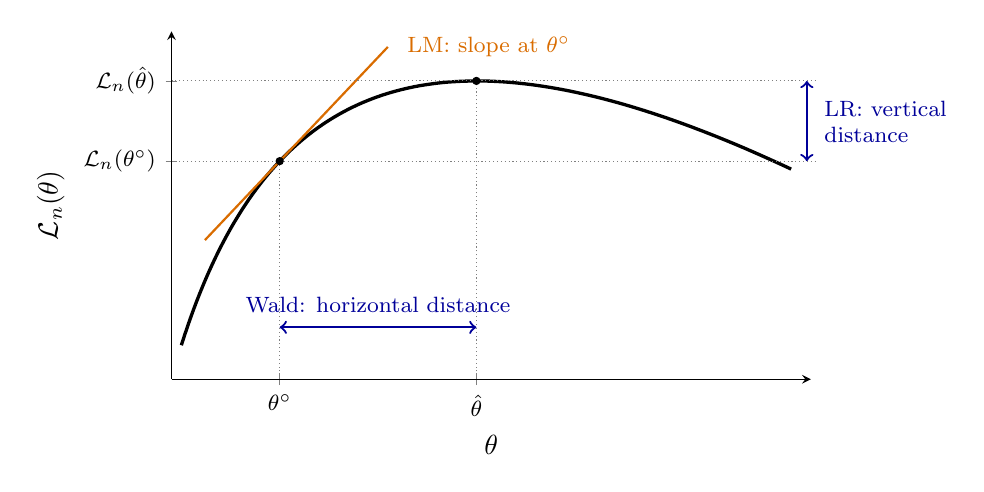
\begin{tikzpicture}
\begin{axis}[
  width=0.8\textwidth, height=6cm,
  xmin=0.45, xmax=3.7, ymin=-4.1, ymax=-0.75,
  axis lines=left, xlabel={$\theta$}, ylabel={$\mathcal{L}_n(\theta)$},
  xtick={1, 2}, xticklabels={$\theta^\circ$, $\hat\theta$},
  ytick={-2, -1.2274}, yticklabels={$\mathcal{L}_n(\theta^\circ)$, $\mathcal{L}_n(\hat\theta)$},
  every tick label/.append style={font=\footnotesize},
  samples=200, domain=0.5:3.6, clip=false]
  \addplot[black, very thick] {4*ln(x) - 2*x};
  \addplot[orange!85!black, thick, domain=0.62:1.55] {-2 + 2*(x - 1)};
  \draw[gray, densely dotted] (axis cs:0.45,-1.2274) -- (axis cs:3.72,-1.2274);
  \draw[gray, densely dotted] (axis cs:0.45,-2) -- (axis cs:3.72,-2);
  \draw[gray, densely dotted] (axis cs:1,-4.1) -- (axis cs:1,-2);
  \draw[gray, densely dotted] (axis cs:2,-4.1) -- (axis cs:2,-1.2274);
  \draw[<->, thick, blue!60!black] (axis cs:3.68,-2) -- (axis cs:3.68,-1.2274);
  \node[font=\footnotesize, anchor=west, text=blue!60!black, align=left] at (axis cs:3.72,-1.62) {LR: vertical\\ distance};
  \draw[<->, thick, blue!60!black] (axis cs:1,-3.6) -- (axis cs:2,-3.6);
  \node[font=\footnotesize, anchor=south, text=blue!60!black, yshift=2pt] at (axis cs:1.5,-3.6) {Wald: horizontal distance};
  \node[font=\footnotesize, anchor=west, text=orange!85!black] at (axis cs:1.6,-0.9) {LM: slope at $\theta^\circ$};
  \fill (axis cs:1,-2) circle (1.5pt);
  \fill (axis cs:2,-1.2274) circle (1.5pt);
\end{axis}
\end{tikzpicture}
\caption[Geometry of the Wald, likelihood ratio and Lagrange multiplier tests]{Geometry of the Wald, likelihood ratio
and Lagrange multiplier tests of $H_0: \theta = \theta^\circ$ for one parameter. The curve is an illustrative
log-likelihood, $\mathcal{L}_n(\theta) = 4\ln\theta - 2\theta$, maximized at $\hat\theta = 2$, with $\theta^\circ = 1$. The
straight segment is the tangent at $\theta^\circ$, whose slope is the score.}
\label{fig:A-trinity}
\end{figure}

The tests differ in what they require. Wald needs only the unrestricted estimate, LM only the restricted one, and LR both.
LM is convenient when the restricted model is easy and the unrestricted one hard, for instance when testing whether a
random coefficient has zero variance starting from logit estimates. Wald is not invariant to how the restriction is
written. Suppose $\hat\theta = 2$ with standard error $0.5$. Writing $H_0$ as $\theta = 1$ gives $\mathcal{W} = (\frac{2 -
1}{0.5})^2 = 4$. Writing it as $\ln\theta = 0$ gives, by the delta method, $\mathcal{W} = (\frac{\ln 2}{0.25})^2 = 7.7$.
Writing it as $\frac{1}{\theta} = 1$ gives $\mathcal{W} = (\frac{0.5}{0.125})^2 = 16$. The likelihood ratio is the same for
all three, because it depends only on the values of the likelihood. In the normal linear regression the three satisfy
$\mathcal{W} \ge \mathcal{LR} \ge \mathcal{LM}$ in every sample \citep{BerndtSavin1977}.

A likelihood ratio test from the book illustrates the mechanics. \citet{PorterZona1993} estimate a ranked logit model of
bids, described in \cref{sec:A-mle-discrete}, three times: on all bid ranks, on the lowest bids only, and on the higher
ranks only.\footnote{We read NBER Working Paper 4013 (March 1992), the working-paper version of \citet{PorterZona1993}.
Table numbers refer to that version.} If the same coefficients govern both parts, the restricted log-likelihood is the
all-ranks value and the unrestricted one is the sum of the two separate values. For competitive firms the log-likelihoods
are $-291.4$, $-89.85$ and $-199.4$ (WP Table 5), so
\begin{equation*}
  \mathcal{LR} = 2\big[(-89.85) + (-199.4) - (-291.4)\big] = 4.3,
\end{equation*}
with six degrees of freedom and a $p$-value of 0.64 (our computation). For cartel members the values are $-73.97$,
$-44.58$ and $-24.92$ (WP Table 6), so $\mathcal{LR} = 8.94$ with four degrees of freedom and a $p$-value of 0.063. Porter and
Zona reject the null of no phantom bidding for the cartel at about the 10 percent level, and they do not reject it for
the competitive firms (\cref{ch:collusion-evidence}).

\Cref{tab:A-tests} collects the tests used in this book.

\begin{table}[htbp]
\centering
\caption{Specification and hypothesis tests used in this book}
\label{tab:A-tests}
\footnotesize
\renewcommand{\arraystretch}{1.15}
\begin{tabularx}{\textwidth}{@{}>{\raggedright\arraybackslash}p{2.1cm}>{\raggedright\arraybackslash}X
>{\raggedright\arraybackslash}p{1.9cm}>{\raggedright\arraybackslash}p{2.2cm}>{\raggedright\arraybackslash}X@{}}
\toprule
Test & Statistic & Null distribution & Estimates needed & Example in the book \\
\midrule
Wald & $n\,a(\hat\theta)^\T[\hat A\hat V\hat A^\T]^{-1}a(\hat\theta)$ & $\chi^2_r$ & unrestricted & equal sugar demand
coefficients across seasons (\cref{ch:conduct}) \\
Likelihood ratio & $2n[\mathcal{L}_n(\hat\theta) - \mathcal{L}_n(\tilde\theta)]$ & $\chi^2_r$ & both & stability of ranked-logit
coefficients across bid ranks (\cref{ch:collusion-evidence}) \\
Lagrange multiplier & $n\,\bar s_n(\tilde\theta)^\T\tilde{\mathcal{I}}^{-1}\bar s_n(\tilde\theta)$ & $\chi^2_r$ & restricted &
zero variance of a random coefficient from logit estimates (\cref{ch:blp}) \\
Hansen $J$ & $n\,\bar g_n(\hat\theta)^\T\hat S^{-1}\bar g_n(\hat\theta)$ & $\chi^2_{L-K}$ & efficient GMM &
overidentifying restrictions in logit and RC logit demand (\cref{app:problems}) \\
Hausman & $(\hat\beta_C - \hat\beta_E)^\T[\hat V_C - \hat V_E]^{-}(\hat\beta_C - \hat\beta_E)$ & $\chi^2$, d.f.\ = rank
of $V_C - V_E$ & efficient and robust & exogeneity of route share and concentration (\cref{ch:airlines}) \\
Anderson-Rubin & $F$ test of $Z$ in a regression of $y - X\beta^\circ$ on $Z$ & $F(L, n - L - K_1)$ under normality &
none & weak-instrument robust confidence sets (\cref{sec:A-weakiv}) \\
First-stage $F$ & $F$ test of excluded instruments in the first stage & noncentral $F$ & first stage & instrument
strength in demand estimation (\cref{sec:A-weakiv}) \\
Cox & centered $\mathcal{LR}$ between non-nested models, standardized & $N(0, 1)$ & both models & collusion against
Bertrand pricing in 1955 autos (\cref{ch:discrete}) \\
Vuong & $\frac{\sqrt{n}\,\overline{LR}}{\hat\omega}$ & $N(0, 1)$ & both models & choosing between non-nested demand or
conduct models \\
Conditional Kolmogorov & $\max_j\sqrt{n}\,\lvert H_n(Z_j) - F_n(Z_j, \hat\theta)\rvert$ & parametric bootstrap &
parametric model & Gamma-Weibull bid distributions in timber auctions (\cref{ch:auction-empirics}) \\
\bottomrule
\end{tabularx}
\par\smallskip
\parbox{\linewidth}{\footnotesize Notes: $r$ is the number of restrictions, $L$ the number of moments and $K$ the number of
parameters. Subscripts $C$ and $E$ denote an estimator consistent under both hypotheses and one efficient under the null. The
superscript $-$ denotes a generalized inverse. In the Anderson-Rubin row, $L$ counts the excluded instruments and $K_1$
the exogenous regressors partialled out.
$\overline{LR}$ is the average pointwise log-likelihood ratio and $\hat\omega$ its standard deviation
(\cref{sec:A-nonnested}). $H_n$ and $F_n$ are defined in \cref{sec:A-ck-test}.}
\end{table}

\subsection{Likelihoods for discrete outcomes}\label{sec:A-mle-discrete}

\casehead{Binary choice}
Let a latent index $y_i^* = x_i^\T\beta + \varepsilon_i$ determine the outcome $y_i = \indic\{y_i^* > 0\}$, with $\varepsilon_i$
independent of $x_i$ and symmetric with distribution function $F$. Then $\Pr(y_i = 1 \mid x_i) = F(x_i^\T\beta)$, and
\begin{equation*}
  \mathcal{L}_n(\beta) = \frac{1}{n}\sum_{i=1}^n\Big[y_i\ln F(x_i^\T\beta) + (1 - y_i)\ln\{1 - F(x_i^\T\beta)\}\Big].
\end{equation*}
The \emph{logit} takes $F = \Lambda$ with $\Lambda(v) = \frac{e^v}{1 + e^v}$, and the \emph{probit} takes $F = \Phi$, the
standard normal distribution function. Only $\frac{\beta}{\sigma_\varepsilon}$ is identified, so the scale of $\varepsilon$ is
normalized (\cref{sec:A-models}). For the logit, $\Lambda'(v) = \Lambda(v)\{1 - \Lambda(v)\}$, so the score and the
Hessian are
\begin{equation}\label{eq:A-logit-score}
  \nabla_\beta\mathcal{L}_n = \frac{1}{n}\sum_i\{y_i - \Lambda(x_i^\T\beta)\}x_i,
  \qquad
  \nabla_{\beta\beta}\mathcal{L}_n = -\frac{1}{n}\sum_i\Lambda(x_i^\T\beta)\{1 - \Lambda(x_i^\T\beta)\}x_ix_i^\T.
\end{equation}

\begin{proposition}[Concavity of the logit likelihood]\label{prop:A-logit-concave}
If $\sum_ix_ix_i^\T$ is positive definite, the binary logit log-likelihood is strictly concave in $\beta$. Hence it has at
most one maximizer, and any solution of the first-order condition is the ML estimator.
\end{proposition}

\begin{proof}
Each weight $\Lambda(1 - \Lambda)$ in \eqref{eq:A-logit-score} lies in $(0, \frac{1}{4}]$. For any $c \ne 0$,
\begin{equation*}
  c^\T\nabla_{\beta\beta}\mathcal{L}_n\,c = -\frac{1}{n}\sum_i\Lambda_i(1 - \Lambda_i)(x_i^\T c)^2 < 0,
\end{equation*}
because $x_i^\T c \ne 0$ for some $i$ when $\sum_ix_ix_i^\T$ is positive definite. A strictly concave function has at most one
maximizer, and a stationary point of a concave function is a global maximizer.
\end{proof}

A maximizer can fail to exist. If some linear combination of the regressors separates the ones from the zeros perfectly,
the likelihood rises without bound along that direction. The probit log-likelihood is also concave, because $\Phi$ and
$1 - \Phi$ are log-concave. \Cref{thm:A-concave} then gives consistency without compactness.

\casehead{Multinomial and conditional logit}
Let consumer $i$ choose one of $J + 1$ alternatives with utilities $u_{ij} = x_{ij}^\T\beta + \epsilon_{ij}$ and $\epsilon_{ij}$
i.i.d.\ type-I extreme value. With $d_{ij} = 1$ if $i$ chooses $j$, the conditional logit of \citet{McFadden1974} has
\begin{equation*}
  P_{ij}(\beta) = \frac{e^{x_{ij}^\T\beta}}{\sum_{k=0}^Je^{x_{ik}^\T\beta}}, \qquad
  \mathcal{L}_n(\beta) = \frac{1}{n}\sum_i\sum_jd_{ij}\ln P_{ij}(\beta).
\end{equation*}
Using $\frac{\partial\ln P_{ij}}{\partial\beta} = x_{ij} - \bar x_i$ with $\bar x_i = \sum_kP_{ik}x_{ik}$,
\begin{equation*}
  \nabla_\beta\mathcal{L}_n = \frac{1}{n}\sum_i\sum_jd_{ij}(x_{ij} - \bar x_i), \qquad
  \nabla_{\beta\beta}\mathcal{L}_n = -\frac{1}{n}\sum_i\sum_jP_{ij}(x_{ij} - \bar x_i)(x_{ij} - \bar x_i)^\T.
\end{equation*}
The Hessian is minus a weighted covariance matrix, so the log-likelihood is concave. With consumer-level data in many
markets, product-market constants $\delta_{jt}$ can be estimated by ML along with the taste-heterogeneity parameters. They
absorb the unobserved quality $\xi_{jt}$. The mean price coefficient is then recovered in a second step,
$\delta_{jt} = x_{jt}\beta - \alpha p_{jt} + \xi_{jt}$, which still needs instruments (\cref{ch:logit,ch:blp}). This is a
two-step estimator in the sense of \cref{sec:A-twostep}.

\casehead{Binomial entry}
\citet{AtheyLevinSeira2011} model the entry of loggers into Forest Service timber auctions. Each of $N_{L,t}$ potential
loggers enters sale $t$ independently with probability $p_L(X_t, N_t) = \Lambda(X_t\alpha_X + N_t\alpha_N)$, where $X_t$ are
sale characteristics and $N_t$ the numbers of potential entrants. The number of entrants is then
$n_{L,t} \sim \mathrm{Binomial}(N_{L,t}, p_L(X_t, N_t))$, and
\begin{equation*}
  \ln L(\alpha) = \sum_t\Big[n_{L,t}\ln p_L(X_t, N_t) + (N_{L,t} - n_{L,t})\ln\{1 - p_L(X_t, N_t)\}\Big] + \text{const}.
\end{equation*}
This is a grouped logit. The score is $\sum_t\{n_{L,t} - N_{L,t}p_L(X_t, N_t)\}(X_t, N_t)^\T$ and the log-likelihood is
concave. They estimate it on $N = 339$ Northern and $N = 382$ California observations. The coefficient on the number of
active loggers is $-0.041$ (0.006) in the North and $-0.050$ (0.007) in California (Table IV). More potential entrants
lower each one's entry probability, as a mixed-strategy entry equilibrium predicts (\cref{ch:auction-empirics}).

\casehead{Rank-ordered logit}
Sometimes we observe a full ranking of alternatives, such as the order of all bids in a procurement auction. Let
$U_j = V_j + \epsilon_j$ with $\epsilon_j$ i.i.d.\ type-I extreme value, $j = 1, \dots, J$.

\begin{proposition}[Rank-ordered logit]\label{prop:A-exploded-logit}
The probability of the ranking $U_{r_1} > U_{r_2} > \dots > U_{r_J}$ is
\begin{equation}\label{eq:A-exploded}
  \Pr(U_{r_1} > U_{r_2} > \dots > U_{r_J}) = \prod_{m=1}^{J}\frac{e^{V_{r_m}}}{\sum_{k=m}^Je^{V_{r_k}}}.
\end{equation}
\end{proposition}

\begin{proof}
The type-I extreme value distribution function is $\Pr(\epsilon \le a) = \exp(-e^{-a})$. Hence $E_j = e^{-\epsilon_j}$ is
exponential with rate one, since $\Pr(e^{-\epsilon_j} > t) = \Pr(\epsilon_j < -\ln t) = e^{-t}$. Define
$T_j = e^{-U_j} = e^{-V_j}E_j$, which is exponential with rate $\lambda_j = e^{V_j}$. The map $u \mapsto e^{-u}$ is
decreasing, so the ranking of the $U$'s from highest to lowest is the ranking of the $T$'s from smallest to largest. For
independent exponentials, $\Pr(T_{r_1} = \min_kT_k) = \frac{\lambda_{r_1}}{\sum_k\lambda_k}$. By the memoryless property, given
that $T_{r_1}$ is the minimum, the excesses $T_k - T_{r_1}$ for $k \ne r_1$ are again independent exponentials with rates
$\lambda_k$, independent of $T_{r_1}$. The ordering of the remaining $T$'s equals the ordering of these excesses, so the
argument repeats on the remaining set. Multiplying the stage probabilities gives \eqref{eq:A-exploded}, with
$\lambda_{r_m} = e^{V_{r_m}}$.
\end{proof}

The ranking likelihood ``explodes'' into a sequence of logit choices from shrinking choice sets
\citep{BeggsCardellHausman1981}. Each auction contributes one product \eqref{eq:A-exploded}, and the sample likelihood is
the product over auctions. Standard multinomial logit software estimates it.

\citet{PorterZona1993} apply the model to bids for highway paving contracts on Long Island, 1979--1985. They approximate the equilibrium bid
function by $\log b_{it} = \alpha_t + X_{it}\beta + \epsilon_{it}$, with an auction effect $\alpha_t$ and an auction-specific
error variance $\sigma_t^2$. They deflate the data by the estimated $\sigma_t$. The probability that firm $i$ submits the
lowest bid is then a multinomial logit in the deflated cost shifters $Z_{it}$, in which the auction effect cancels:
\begin{equation*}
  \Pr(b_{it} < b_{jt}\ \forall j \ne i) = \frac{e^{\beta Z_{it}}}{\sum_je^{\beta Z_{jt}}}.
\end{equation*}
The low bid is the ``most preferred'' alternative, so with $r_m$ the firm whose bid is ranked $m$-th lowest among $n_t$ bids,
\eqref{eq:A-exploded} gives the likelihood $L(\beta) = \prod_t\prod_{i=1}^{n_t}\frac{e^{\beta Z_{r_it}}}{\sum_{j=i}^{n_t}e^{\beta Z_{r_jt}}}$.
The model follows from the bid equation if minus the bid error is type-I extreme value (WP pp.~24--25). The product splits
into the factor for the lowest bid ($i = 1$) and the factors for the higher ranks ($i \ge 2$). Under the model both parts
identify the same $\beta$. Phantom bids by cartel members, placed above the designated winner's bid, need not reflect costs.
The likelihood ratio test of equal coefficients computed above therefore detects them, with the competitive firms as a
check on the specification \citep{HausmanRuud1987}.

\subsection{Latent variables}\label{sec:A-mle-latent}

Many IO models contain variables that the firms observe and the econometrician does not: an auction-level shock common
to all bidders, or the regime of a cartel. The likelihood of the data integrates the latent variable out,
\begin{equation*}
  f(y \mid x;\theta) = \int f(y \mid x, u;\theta)\,\dd F(u \mid x;\theta).
\end{equation*}
Three cases arise in this book: an integral with a closed form, a finite mixture, and a hidden Markov chain.

\subsubsection*{Closed-form heterogeneity: Gamma-Weibull bids}

\citet{AtheyLevinSeira2011} find that sealed bids in the same timber auction are highly correlated given observed sale
characteristics. Following \citet{Krasnokutskaya2011}, they let an auction characteristic $u$, known to the bidders but not
to the econometrician, shift all bids. Conditional on $(X, u, N, n)$, the bid of a bidder of type $k \in \{L, M\}$ (logger or
mill) is Weibull (journal p.~237, eq.~8):
\begin{equation}\label{eq:A-weibull}
  G_k(b \mid X, u, N, n) = 1 - \exp\left\{-u\left(\frac{b}{\lambda_k(X, N, n)}\right)^{\rho_k(n)}\right\}.
\end{equation}
The scale satisfies $\ln\lambda_k = X\beta_X + N\beta_N + n\beta_{n,k} + \beta_{0,k}$ and the shape satisfies
$\ln\rho_k = n\gamma_{n,k} + \gamma_{0,k}$. The heterogeneity $u$ is Gamma with mean one and variance $\sigma_u^2$,
independent of $(X, N, n)$. Athey, Levin and Seira (ALS) denote this variance by $\theta$. Bids are independent given $u$. A large $u$ lowers every
bid in the auction by the common factor $u^{-\frac{1}{\rho_k}}$, since \eqref{eq:A-weibull} says that $u^{\frac{1}{\rho_k}}b$
is Weibull with parameters $(\lambda_k, \rho_k)$ whatever $u$ is.

\begin{proposition}[Closed-form auction likelihood]\label{prop:A-gamma-weibull}
Let auction $t$ have the set of participants $\mathcal{N}_t$, with $\lvert\mathcal{N}_t\rvert = n$ bids $b_i$, and write
$z_i = (\frac{b_i}{\lambda_{k(i)}})^{\rho_{k(i)}}$. The joint density of the bids is
\begin{equation}\label{eq:A-gw-lik}
  \ell_t = \prod_{i \in \mathcal{N}_t}\left[\frac{\rho_{k(i)}}{\lambda_{k(i)}}\left(\frac{b_i}{\lambda_{k(i)}}\right)^{\rho_{k(i)} - 1}\right]
  \frac{\Gamma\big(n + \frac{1}{\sigma_u^2}\big)}{\Gamma\big(\frac{1}{\sigma_u^2}\big)\,
  \big(\sigma_u^2\big)^{\frac{1}{\sigma_u^2}}\,\big(\sum_{i \in \mathcal{N}_t}z_i + \frac{1}{\sigma_u^2}\big)^{n + \frac{1}{\sigma_u^2}}}.
\end{equation}
\end{proposition}

\begin{proof}
Differentiating \eqref{eq:A-weibull}, the density of one bid given $u$ is
\begin{equation*}
  g_k(b \mid u) = u\,\frac{\rho_k}{\lambda_k}\left(\frac{b}{\lambda_k}\right)^{\rho_k - 1}e^{-uz}, \qquad
  z = \left(\frac{b}{\lambda_k}\right)^{\rho_k}.
\end{equation*}
Given $u$ the bids are independent, so their joint density is
\begin{equation*}
  u^{n}\prod_{i \in \mathcal{N}_t}\left[\frac{\rho_{k(i)}}{\lambda_{k(i)}}\left(\frac{b_i}{\lambda_{k(i)}}\right)^{\rho_{k(i)} -
  1}\right]\exp\Big(-u\sum_{i \in \mathcal{N}_t}z_i\Big).
\end{equation*}
A Gamma variable with mean one and variance $\sigma_u^2$ has shape $a = \frac{1}{\sigma_u^2}$, scale
$\sigma_u^2$, and density $\frac{u^{a-1}e^{-\frac{u}{\sigma_u^2}}}{\Gamma(a)(\sigma_u^2)^a}$. Integrating $u$ out leaves
\begin{equation*}
  \frac{1}{\Gamma(a)(\sigma_u^2)^a}\int_0^\infty u^{n + a - 1}
  \exp\left\{-u\left(\sum_iz_i + \frac{1}{\sigma_u^2}\right)\right\}\dd u
  = \frac{\Gamma(n + a)}{\Gamma(a)(\sigma_u^2)^a\big(\sum_iz_i + \frac{1}{\sigma_u^2}\big)^{n + a}},
\end{equation*}
by the Gamma integral $\int_0^\infty u^{c-1}e^{-du}\,\dd u = \frac{\Gamma(c)}{d^c}$. Multiplying by the product term gives
\eqref{eq:A-gw-lik}.
\end{proof}

The Gamma mixing distribution is conjugate to the exponential kernel in \eqref{eq:A-weibull}, which is why the integral has a
closed form. ALS write their likelihood in an online appendix (journal p.~238). The expression above is our derivation
from their specification. They estimate it on sales with at least two bidders (Table IV notes). The estimates of
$\ln\sigma_u^2$ are $-0.502$ (0.120) in the Northern sales and $-0.416$ (0.124) in California (Table IV). These imply
$\sigma_u^2 = 0.61$ and $0.66$, with delta-method standard errors of 0.07 and 0.08 (our computation). Auction
heterogeneity is substantial. The fitted model reproduces the moments of normalized bids. In the North the data show a
mean of 2.16, a standard deviation of 1.18, a between-auction standard deviation of 0.94 and a within-auction standard
deviation of 0.75. The model predicts 2.12, 1.21, 0.97 and 0.70 (journal p.~238). When no conjugate pair exists, the
integral is computed by quadrature or simulation (\cref{sec:A-simulation}).

\subsubsection*{Finite mixtures and switching regressions: the JEC cartel}

\citet{Porter1983} studies the Joint Executive Committee (JEC), a legal railroad cartel that set rates for grain shipped
east from Chicago. The data are weekly from 1880 to 1886, 328 observations. The cartel alternated between collusive
periods and price wars, and the econometrician does not know with certainty which weeks were which. Let $Q_t$ be the
tonnage shipped, $p_t$ the grain rate and $L_t$ a dummy for the Great Lakes being open to navigation. Let $S_t$ collect
dummies for entry and acquisitions and $I_t$ indicate the collusive regime. The model is (journal pp.~304--305)
\begin{align}
  \log Q_t &= \alpha_0 + \alpha_1\log p_t + \alpha_2L_t + U_{1t},\label{eq:A-porter-demand}\\
  \log p_t &= \beta_0 + \beta_1\log Q_t + \beta_2S_t + \beta_3I_t + U_{2t}.\label{eq:A-porter-supply}
\end{align}
The errors $U_t = (U_{1t}, U_{2t})^\T$ are i.i.d.\ $N(0, \Sigma)$. Twelve four-week seasonal dummies enter both equations
and are suppressed here. The regime shifts only the intercept of the supply relation. Porter derives
\eqref{eq:A-porter-supply} from firm first-order conditions $p_t(1 + \frac{\theta_t}{\alpha_1}) = MC_i(q_{it})$. If price wars
are Bertrand and collusive periods have constant conduct $\theta$, then $\beta_3 = -\ln(1 + \frac{\theta}{\alpha_1})$.

Write the system as $By_t = \Gamma X_t + \Delta I_t + U_t$ with $y_t = (\log Q_t, \log p_t)^\T$, $X_t = (1, L_t, S_t^\T)^\T$ and
\begin{equation*}
  B = \begin{pmatrix} 1 & -\alpha_1 \\ -\beta_1 & 1\end{pmatrix}, \qquad
  \Delta = \begin{pmatrix} 0 \\ \beta_3\end{pmatrix}, \qquad
  \Gamma = \begin{pmatrix} \alpha_0 & \alpha_2 & 0 \\ \beta_0 & 0 & \beta_2^\T\end{pmatrix}.
\end{equation*}
Given $I_t$, the change of variables from $U_t$ to $y_t$ has Jacobian $\lvert\det B\rvert = \lvert 1 - \alpha_1\beta_1\rvert$, so
\begin{equation}\label{eq:A-porter-h}
  h(y_t \mid I_t) = (2\pi)^{-1}\lvert\Sigma\rvert^{-\frac{1}{2}}\lvert\det B\rvert
  \exp\left\{-\frac{1}{2}(By_t - \Gamma X_t - \Delta I_t)^\T\Sigma^{-1}(By_t - \Gamma X_t - \Delta I_t)\right\}.
\end{equation}
If the regimes are known, 2SLS or ML with $I_t$ as data is straightforward. Porter instead treats $I_t$ as an i.i.d.
Bernoulli variable with $\Pr(I_t = 1) = \lambda$. The density of $y_t$ is then a two-component mixture, and the likelihood is
(journal p.~306, eq.~5)
\begin{equation}\label{eq:A-mixture}
  L(\Omega, \lambda) = \prod_{t=1}^T\big[\lambda h(y_t \mid 1) + (1 - \lambda)h(y_t \mid 0)\big],
\end{equation}
with $\Omega = (B, \Gamma, \Delta, \Sigma)$.

Mixture likelihoods are awkward to maximize directly, because the log of a sum does not separate. The
\emph{expectation-maximization} (EM) algorithm of \citet{DempsterLairdRubin1977} exploits the fact that the likelihood
would be easy if the regimes were observed. The complete-data log-likelihood is
\begin{equation*}
  \ln L^c(\Omega, \lambda) = \sum_t\Big[I_t\{\ln\lambda + \ln h(y_t \mid 1)\} + (1 - I_t)\{\ln(1 - \lambda) + \ln h(y_t \mid 0)\}\Big].
\end{equation*}
Starting from $(\Omega^{(m)}, \lambda^{(m)})$, iterate two steps.
\begin{enumerate}
  \item \emph{E step.} Compute the posterior probability of collusion in each week by Bayes' rule,
  \begin{equation}\label{eq:A-estep}
    w_t^{(m)} = \Pr(I_t = 1 \mid y_t;\Omega^{(m)}, \lambda^{(m)}) =
    \frac{\lambda^{(m)}h(y_t \mid 1;\Omega^{(m)})}{\lambda^{(m)}h(y_t \mid 1;\Omega^{(m)}) + (1 - \lambda^{(m)})h(y_t \mid 0;\Omega^{(m)})}.
  \end{equation}
  \item \emph{M step.} Maximize the expected complete-data log-likelihood, which replaces $I_t$ by $w_t^{(m)}$ in
  $\ln L^c$. This gives $\lambda^{(m+1)} = \frac{1}{T}\sum_tw_t^{(m)}$ and
  \begin{equation*}
    \Omega^{(m+1)} = \argmax_\Omega\sum_t\Big[w_t^{(m)}\ln h(y_t \mid 1;\Omega) + (1 - w_t^{(m)})\ln h(y_t \mid 0;\Omega)\Big],
  \end{equation*}
  a weighted full-information ML problem.
\end{enumerate}
Porter adapts the version of this algorithm proposed by \citet{Kiefer1980} for switching regressions. He stops when the
correlation between successive $w_t$ series exceeds .999 (journal p.~306).

A detail of the M step deserves care. The weighted objective is not the known-regime likelihood with $w_t$ substituted for
$I_t$. Write $e_t = By_t - \Gamma X_t$. The expected complete-data log-likelihood weights the quadratic forms of the two
regimes by $w_t$ and $1 - w_t$, and completing the square gives
\begin{equation*}
  w_t(e_t - \Delta)^\T\Sigma^{-1}(e_t - \Delta) + (1 - w_t)e_t^\T\Sigma^{-1}e_t
  = (e_t - w_t\Delta)^\T\Sigma^{-1}(e_t - w_t\Delta) + w_t(1 - w_t)\Delta^\T\Sigma^{-1}\Delta.
\end{equation*}
The plug-in shortcut drops the last term, which matters when posterior probabilities are far from zero and one. In the
simulated example below, the shortcut converges to $\hat\beta_3 = 0.618$, with a mixture log-likelihood 5.7 points below the
maximum attained by exact EM.

\begin{proposition}[EM never lowers the likelihood]\label{prop:A-em-monotone}
Let $\vartheta = (\Omega, \lambda)$ and let $\vartheta^{(m+1)}$ maximize
$\mathcal{Q}(\vartheta \mid \vartheta^{(m)}) = \E[\ln L^c(\vartheta) \mid y;\vartheta^{(m)}]$. Then
$\ln L(\vartheta^{(m+1)}) \ge \ln L(\vartheta^{(m)})$.
\end{proposition}

\begin{proof}
Let $k(I \mid y;\vartheta)$ be the conditional probability of the regime sequence $I$ given the data. By the definition of
conditional probability, $\ln L(\vartheta) = \ln L^c(\vartheta) - \ln k(I \mid y;\vartheta)$ for every $I$. Take the expectation
over $I$ under $k(\cdot \mid y;\vartheta^{(m)})$. The left side does not depend on $I$, so
\begin{equation*}
  \ln L(\vartheta) = \mathcal{Q}(\vartheta \mid \vartheta^{(m)}) - \mathcal{H}(\vartheta \mid \vartheta^{(m)}),
  \qquad
  \mathcal{H}(\vartheta \mid \vartheta^{(m)}) = \E[\ln k(I \mid y;\vartheta) \mid y;\vartheta^{(m)}].
\end{equation*}
By \cref{lem:A-info-inequality} applied to the conditional distribution of $I$, $\mathcal{H}(\vartheta \mid \vartheta^{(m)}) \le
\mathcal{H}(\vartheta^{(m)} \mid \vartheta^{(m)})$ for every $\vartheta$. The M step gives $\mathcal{Q}(\vartheta^{(m+1)} \mid
\vartheta^{(m)}) \ge \mathcal{Q}(\vartheta^{(m)} \mid \vartheta^{(m)})$. Hence
\begin{align*}
  \ln L(\vartheta^{(m+1)}) - \ln L(\vartheta^{(m)})
  &= \big[\mathcal{Q}(\vartheta^{(m+1)} \mid \vartheta^{(m)}) - \mathcal{Q}(\vartheta^{(m)} \mid \vartheta^{(m)})\big] \\
  &\quad - \big[\mathcal{H}(\vartheta^{(m+1)} \mid \vartheta^{(m)}) - \mathcal{H}(\vartheta^{(m)} \mid \vartheta^{(m)})\big]
  \ge 0. \qedhere
\end{align*}
\end{proof}

The proof also shows that the gradient of $\mathcal{H}(\cdot \mid \vartheta^{(m)})$ is zero at $\vartheta^{(m)}$. So a fixed point
of EM is a stationary point of the observed likelihood. It need not be the global maximum. Convergence is linear, and slow
when the regimes carry much missing information. EM does not deliver standard errors. They come from the observed
information of the mixture likelihood \eqref{eq:A-mixture} at the EM solution \citep{Louis1982}.

After estimation each week is classified as collusive if $\hat w_t > .5$. The rule minimizes the expected number of
misclassified weeks \citep{LeePorter1984}. The expected number of errors of a classification $\hat I_t$ is
$\sum_t[\hat I_t(1 - \hat w_t) + (1 - \hat I_t)\hat w_t]$, and each term is minimized by choosing $\hat I_t = 1$ exactly when
$\hat w_t > 1 - \hat w_t$.

Porter compares 2SLS with a regime series reported in the trade press (the PO series) and ML with the estimated series (PN).
The demand estimates are almost identical, with price elasticities of $-.742$ (.121) and $-.800$ (.091). The regime
coefficient $\hat\beta_3$ rises from .382 (.059) under 2SLS to .545 (.032) under ML. It is larger and has about half the
standard error. The $R^2$ of the supply relation rises from .320 to .863 (Table 3). The implied conduct parameter is
\begin{equation*}
  \hat\theta = \hat\alpha_1\big(e^{-\hat\beta_3} - 1\big) = -0.800\times\big(e^{-0.545} - 1\big) = 0.336,
\end{equation*}
which Porter calls roughly consistent with Cournot behavior in collusive periods (journal p.~309). At sample means,
collusive weeks have prices about 66 percent higher, quantities about 33 percent lower and revenues about 11 percent
higher than price-war weeks (Table 4, p.~310). The full table and its interpretation are in \cref{ch:collusion-evidence}.

\Cref{fig:A-em} applies the algorithm to simulated data with the same structure. Demand and supply parameters are set near
Porter's ML estimates, and the regime follows a Markov chain with the transition probabilities that \citet{Ellison1994}
estimates. The simulated sample has six price wars covering 65 of 328 weeks. Exact EM from a median split of the supply
residuals converges in 25 iterations to $\hat\beta_3 = 0.563$ (0.030), against the true 0.545. The correlation between
successive $w_t$ series first exceeds .999 at iteration 10. The rule $\hat w_t > .5$ misclassifies 11 weeks. The
log-likelihood rises at every iteration, as \cref{prop:A-em-monotone} requires. A random starting classification shows the
other side of the proposition. It carries no information about the regimes, so the first M step sets $\hat\beta_3$ close to
zero. With equal regime densities every posterior equals $\lambda$, and the algorithm stays at this degenerate fixed point,
37.3 log points below the maximum (\cref{fig:A-em}, panel a).

\begin{figure}[htbp]
\centering
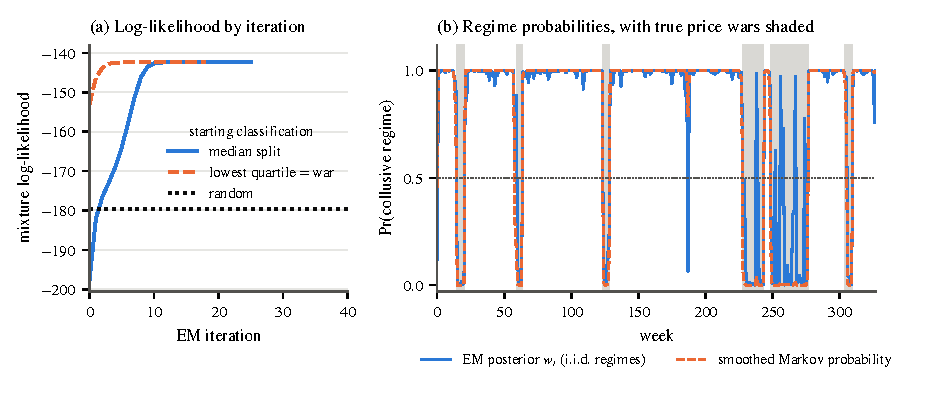
\includegraphics[width=\textwidth]{figures/appA/em_switching.pdf}
\caption[EM and Markov-switching estimation of a simulated two-regime supply relation]{EM and Markov-switching
estimation of a simulated two-regime supply relation. The design is \eqref{eq:A-porter-demand} and
\eqref{eq:A-porter-supply} with $T = 328$, $(\alpha_0, \alpha_1, \alpha_2) = (9.09, -0.80, -0.43)$, $(\beta_0, \beta_1, \beta_2, \beta_3) = (-2.70, 0.09,
-0.20, 0.545)$, one entry dummy, independent errors with standard deviations 0.40 and 0.16, and a Markov regime with
$\Pr(I_{t+1} = 1 \mid I_t = 1) = 0.975$ and $\Pr(I_{t+1} = 1 \mid I_t = 0) = 0.067$. (a) Mixture log-likelihood
by EM iteration from three starting classifications. (b) Posterior probabilities of collusion from the i.i.d.
mixture (EM) and smoothed probabilities from the Markov-switching model estimated by the Hamilton filter. Source:
\texttt{figures/appA/src/em\_switching.py}, seed 20261022.}
\label{fig:A-em}
\end{figure}

\subsubsection*{Hidden Markov models: Ellison's re-estimation}

Porter's i.i.d.\ regimes ignore the persistence of price wars. \citet{Ellison1994} re-estimates the JEC model with two
changes (journal p.~40). First, the demand error follows an AR(1) process, $U_{1t} = \rho U_{1,t-1} + V_{1t}$ with
$\lvert\rho\rvert < 1$, where $\rho$ now denotes an autoregressive coefficient. Second, the regime follows a Markov chain whose
transition probabilities are logits,
\begin{equation}\label{eq:A-ellison-transition}
  \Pr(I_{t+1} = 1 \mid I_t, Z_t) = \frac{e^{\gamma^\T W_t}}{1 + e^{\gamma^\T W_t}},
\end{equation}
where $Z_t$ is the set of predetermined variables at $t$ and $W_t$ contains functions of $I_t$ and of $Z_t$. With $W_t$
equal to a separate constant for each value of $I_t$, the chain is a first-order Markov process. Adding market-share or
demand variables to $W_t$ tests what triggers price wars. Ellison maximizes the joint likelihood of the structural
equations and of the path of transitions.

The likelihood of a hidden Markov model is computed by the filter of \citet{Hamilton1989}. Let $\mathcal{F}_t$ be the data
up to week $t$, and let $h_k(y_t) = f(y_t \mid I_t = k, \mathcal{F}_{t-1})$ be the density of week $t$'s data in regime $k$.
In Ellison's model, $h_k$ is \eqref{eq:A-porter-h} with $U_{1t}$ replaced by $V_{1t} = U_{1t} - \rho U_{1,t-1}$. Write
$p_{k,t} = \Pr(I_{t+1} = 1 \mid I_t = k, Z_t)$, the predicted probability $\xi_{t \mid t-1} = \Pr(I_t = 1 \mid \mathcal{F}_{t-1})$,
and the filtered probability $\xi_{t \mid t} = \Pr(I_t = 1 \mid \mathcal{F}_t)$.

\begin{proposition}[Hamilton filter]\label{prop:A-hamilton}
Suppose $y_t$ depends on the regime history only through $I_t$, given $\mathcal{F}_{t-1}$, and the regime follows
\eqref{eq:A-ellison-transition}. Then for $t = 1, \dots, T$,
\begin{align}
  f(y_t \mid \mathcal{F}_{t-1}) &= \xi_{t \mid t-1}h_1(y_t) + (1 - \xi_{t \mid t-1})h_0(y_t),\label{eq:A-ham-pred}\\
  \xi_{t \mid t} &= \frac{\xi_{t \mid t-1}h_1(y_t)}{f(y_t \mid \mathcal{F}_{t-1})},\label{eq:A-ham-update}\\
  \xi_{t+1 \mid t} &= p_{1,t}\,\xi_{t \mid t} + p_{0,t}\,(1 - \xi_{t \mid t}),\label{eq:A-ham-forecast}
\end{align}
and the log-likelihood is $\ln L = \sum_{t=1}^T\ln f(y_t \mid \mathcal{F}_{t-1})$.
\end{proposition}

\begin{proof}
Equation \eqref{eq:A-ham-pred} is the law of total probability over the two values of $I_t$ given $\mathcal{F}_{t-1}$. Equation
\eqref{eq:A-ham-update} is Bayes' rule, $\Pr(I_t = 1 \mid y_t, \mathcal{F}_{t-1}) = \frac{\Pr(I_t = 1 \mid \mathcal{F}_{t-1})
f(y_t \mid I_t = 1, \mathcal{F}_{t-1})}{f(y_t \mid \mathcal{F}_{t-1})}$. Equation \eqref{eq:A-ham-forecast} again applies the law of
total probability, now over $I_t$ given $\mathcal{F}_t$, using that the transition depends on $\mathcal{F}_t$ only through
$(I_t, Z_t)$. Finally, the joint density of $(y_1, \dots, y_T)$ factors into one-step predictive densities,
$f(y_1, \dots, y_T) = \prod_tf(y_t \mid \mathcal{F}_{t-1})$.
\end{proof}

The recursion needs a starting value $\xi_{1 \mid 0}$, usually the stationary probability $\frac{p_0}{1 - p_1 + p_0}$ when the
transition probabilities are constant. Probabilities that use the whole sample come from a backward pass
\citep{Kim1994}:
\begin{equation*}
  \Pr(I_t = 1 \mid \mathcal{F}_T) = \xi_{t \mid t}\left[p_{1,t}\frac{\Pr(I_{t+1} = 1 \mid \mathcal{F}_T)}{\xi_{t+1 \mid t}} +
  (1 - p_{1,t})\frac{\Pr(I_{t+1} = 0 \mid \mathcal{F}_T)}{1 - \xi_{t+1 \mid t}}\right].
\end{equation*}
In the simulated data of \cref{fig:A-em}, the Markov-switching model estimated by maximizing this likelihood gives
$\Pr(I_{t+1} = 1 \mid I_t = 1) = 0.975$ and $\Pr(I_{t+1} = 1 \mid I_t = 0) = 0.099$, against the true 0.975 and 0.067. The
smoothed probabilities misclassify 5 weeks, against 11 for the i.i.d.\ mixture. Using the persistence of regimes sharpens
the classification of short-lived deviations.

Ellison's estimates (Table 2) give regime constants of 3.675 (.474) after a collusive week and $-2.641$ (.404) after a price
war week. A collusive week is followed by another with probability $\frac{e^{3.675}}{1 + e^{3.675}} = .975$. A price war week
is followed by collusion with probability only $\frac{e^{-2.641}}{1 + e^{-2.641}} = .067$, so wars persist with probability
.933 per week. The implied mean durations are about 40 weeks for collusive spells and 15 weeks for wars, and the stationary
share of collusive weeks is .73 (our computation). Dependence also moves the structural estimates. Allowing AR(1) demand
errors, with $\hat\rho = .832$ (.085), raises the estimated demand elasticity from .84 to 1.80 (journal p.~42). Porter's
approximation to the degree of collusion, $\hat\alpha_1(e^{-\hat\beta_3} - 1)$, rises from .40 to .85. The estimated elasticity is
imprecise, with a standard error of 1.29. The log-likelihood rises from 37.2 to 181.0. If both values are computed on the
same 328 weeks, the implied likelihood ratio statistic for $\rho = 0$ is 287.6 (our computation).

Ellison then adds candidate triggers to $W_t$ in the transition from collusion to war (Table 3). An unusually high market
share for one firm (BIGSHARE1) enters with coefficient $-.77$ (.49), and the unanticipated demand shock $V_{1t}$ with $-4.15$
(2.64). Both have the predicted sign and are significant at about the 6 percent level in one-tailed tests. With only six
price wars in the sample, these tests have little power. \Cref{ch:collusion-evidence} discusses what they imply for the
theories of \citet{GreenPorter1984} and \citet{RotembergSaloner1986}. The econometric point is that joint ML of the regimes,
the transitions and the structural equations uses the timing of every war. A two-step procedure that first classifies weeks
and then regresses the classification on triggers may lose power through misclassification at the onset of wars
(journal p.~39).

\subsection{Non-regular problems}\label{sec:A-mle-nonregular}

The standard theory assumes that the support of the data does not depend on $\theta$, that $\theta_0$ is interior, and that
the likelihood is smooth. Each assumption fails in some IO application, and each failure changes the asymptotics.

\begin{proposition}[Parameter-dependent support]\label{prop:A-uniform-mle}
Let $X_1, \dots, X_n$ be i.i.d.\ uniform on $[0, \theta_0]$. The ML estimator is $\hat\theta = \max_iX_i$, and
\begin{equation*}
  \frac{n(\theta_0 - \hat\theta)}{\theta_0} \xrightarrow{d} \mathrm{Exponential}(1).
\end{equation*}
\end{proposition}

\begin{proof}
The likelihood is $\theta^{-n}\indic\{\theta \ge \max_iX_i\}$, which is zero below the sample maximum and decreasing above it.
So $\hat\theta = \max_iX_i$. For $0 \le t \le n$,
\begin{equation*}
  \Pr\left(\frac{n(\theta_0 - \hat\theta)}{\theta_0} > t\right) = \Pr\left(\max_iX_i < \theta_0\left(1 - \frac{t}{n}\right)\right)
  = \left(1 - \frac{t}{n}\right)^n \to e^{-t}. \qedhere
\end{equation*}
\end{proof}

The estimator converges at rate $n$, faster than $\sqrt{n}$, and its limit is not normal. It is biased downward, with
$\E[\hat\theta] = \frac{n}{n + 1}\theta_0$. The information equality fails because the support moves with $\theta$. The
derivative of $\ln f = -\ln\theta$ is $-\frac{1}{\theta}$, whose mean is not zero. The same structure arises in first-price
auctions, where the upper end of the bid support depends on the parameters of the value distribution.
\citet{DonaldPaarsch1996} develop estimators and tests for this case based on extreme order statistics
(\cref{ch:auction-empirics}). \Cref{prop:A-boot-max} shows that the nonparametric bootstrap fails here.

\begin{proposition}[A parameter on the boundary]\label{prop:A-boundary}
Let $\theta$ be scalar with $\Theta = [0, \infty)$ and $\theta_0 = 0$. Suppose the log-likelihood extends smoothly to a
neighborhood of zero, where the unconstrained maximizer $\hat\theta_u$ satisfies $\sqrt{n}\,\hat\theta_u \xrightarrow{d}
N(0, \mathcal{I}^{-1})$. Then the likelihood ratio statistic for $H_0: \theta = 0$ converges in distribution to an equal mixture
of a point mass at zero and a $\chi^2_1$.
\end{proposition}

\begin{proof}
A second-order expansion around zero, with $\bar s_n(0) = \mathcal{I}\hat\theta_u + o_p(n^{-\frac{1}{2}})$, gives uniformly in
$\theta$ of order $n^{-\frac{1}{2}}$,
\begin{equation*}
  2n\big[\mathcal{L}_n(\theta) - \mathcal{L}_n(0)\big] = n\mathcal{I}\big(2\theta\hat\theta_u - \theta^2\big) + o_p(1).
\end{equation*}
Maximize over $\theta \ge 0$. If $\hat\theta_u > 0$ the maximum is at $\theta = \hat\theta_u$, with value $n\mathcal{I}\hat\theta_u^2$.
If $\hat\theta_u \le 0$ the maximum is at $\theta = 0$, with value zero. So $\mathcal{LR} = (\max\{0, Z_n\})^2 + o_p(1)$ with
$Z_n = \sqrt{n\mathcal{I}}\,\hat\theta_u \xrightarrow{d} N(0, 1)$. Half the time $Z_n \le 0$ and the statistic is zero. Otherwise it is
the square of a standard normal.
\end{proof}

The 5 percent cutoff of this mixture is the 90th percentile of $\chi^2_1$, 2.71, not the usual 3.84
\citep{Chernoff1954, SelfLiang1987, Andrews2001}. Zero variances of random coefficients and zero regime probabilities are
boundary nulls of this kind. Testing the number of regimes is harder still. In Porter's model \eqref{eq:A-mixture} the
null of a single regime can be written in two ways. If $\lambda = 0$, then $\lambda$ lies on the boundary and $\beta_3$ is
not identified, because it multiplies a regime that never occurs. The case $\lambda = 1$ is symmetric. Then $I_t = 1$ in every
week, so $\beta_3$ cannot be separated from the intercept $\beta_0$. If $\beta_3 = 0$, the two mixture components coincide,
and $\lambda$ is not identified. In both cases a parameter is identified only under the alternative. The likelihood ratio
then has no $\chi^2$ limit \citep{Davies1977}, and \citet{Hansen1992} develops bounds for Markov-switching models.

Porter's own test shows the problem at work. He maximizes the likelihood once with switching and once subject to
$\Delta = 0$, which in \eqref{eq:A-porter-supply} means $\beta_3 = 0$. Let $\bar L_1$ and $\bar L_0$ be the two maximized
average log-likelihoods. He reports $2T(\bar L_1 - \bar L_0) = 554.1$, refers it to a $\chi^2_1$ distribution, and
rejects ``the hypothesis that no switch occurred'' (journal p.~312). Under $\Delta = 0$ the mixture density
$\lambda h(y_t \mid 1) + (1 - \lambda)h(y_t \mid 0)$ equals $h(y_t \mid 0)$ for every $\lambda$. The restricted
likelihood is therefore flat in $\lambda$, and the unrestricted fit chooses $\lambda$ and $\beta_3$ together. The
statistic is the largest of a family of likelihood ratios indexed by $\lambda$. Its null distribution is stochastically
larger than $\chi^2_1$, and the $\chi^2_1$ reference is invalid. The size of the statistic still settles the question in
practice. The 0.1 percent cutoff of $\chi^2_1$ is 10.83, and 554.1 is about fifty times larger, so the rejection very
likely survives any valid correction. Porter also notes that $\hat\beta_3$ is significantly positive (journal p.~311). A
$t$ test of $\beta_3 = 0$ faces the same difficulty, because it is computed at an estimate $\hat\lambda$ that has no
limit under the null.

A discontinuous likelihood is the third failure. \citet{Bresnahan1987} solves the vertical model for equilibrium prices
and quantities, adds independent normal errors to observed prices and quantities, and maximizes the resulting likelihood
(\cref{sec:06-bres-estimation}). The likelihood jumps when two products swap positions in the quality ordering. The derivative-based expansion of \cref{thm:A-asy-normal}
is unavailable at the jumps. Estimation then relies on derivative-free search, and asymptotic theory requires the true
parameter to lie away from the discontinuities.

\subsection{Non-nested tests}\label{sec:A-nonnested}

Two models are \emph{non-nested} when neither is a special case of the other. Collusion and Bertrand pricing with the same
demand system are an example (\cref{sec:06-bres-cox}). The likelihood ratio does not have a $\chi^2$ distribution in this
case, and its sign alone is uninformative. Two approaches are standard.

Let model $F$ have density $f(y \mid x;\theta)$ and model $G$ density $g(y \mid x;\gamma)$, with ML estimates $\hat\theta$ and
$\hat\gamma$. Write the pointwise log-likelihood ratio as $d_i = \ln f(y_i \mid x_i;\hat\theta) - \ln g(y_i \mid x_i;\hat\gamma)$
and $LR_n = \sum_id_i$.

The test of \citet{Cox1961, Cox1962} takes $F$ as the null. If $F$ is true with parameter $\theta$, the estimator
$\hat\gamma$ converges to a pseudo-true value $\gamma(\theta)$, and $\frac{1}{n}LR_n$ converges to
$\E_\theta[\ln f(y \mid x;\theta) - \ln g(y \mid x;\gamma(\theta))]$. Cox's statistic centers $LR_n$ by a consistent estimate of
this expectation, computed under $F$ at $\hat\theta$, and divides by an estimate of its standard deviation. Under $F$ it is
asymptotically standard normal. A large negative value says that $G$ fits better than $F$ would lead us to expect. The roles
are then reversed. There are four possible outcomes: reject neither, reject one of the two, or reject both. Rejecting both is
informative, because it says that neither model is adequate. \Cref{prop:06-bres-cox} gives the statistic for nonlinear
regressions with normal errors, and \cref{tab:06-bres-cox} reports Bresnahan's tests of conduct in the 1955 automobile market.

The test of \citet{Vuong1989} treats the models symmetrically. It asks which model is closer to the truth in
Kullback-Leibler divergence.

\begin{proposition}[Vuong's model selection test]\label{prop:A-vuong}
Let $\theta^*$ and $\gamma^*$ be the pseudo-true values of the two models. Suppose $\Pr\{f(y \mid x;\theta^*) \ne g(y \mid
x;\gamma^*)\} > 0$, so that the models are strictly non-nested, and let $\hat\omega^2 = \frac{1}{n}\sum_i(d_i - \bar d)^2$ with
$\bar d = \frac{1}{n}LR_n$. Under $H_0: \E[\ln f(y \mid x;\theta^*) - \ln g(y \mid x;\gamma^*)] = 0$ and standard regularity
conditions,
\begin{equation*}
  T_V = \frac{\sqrt{n}\,\bar d}{\hat\omega} \xrightarrow{d} N(0, 1).
\end{equation*}
\end{proposition}

\begin{proof}[Proof sketch]
Let $\bar d^* = \frac{1}{n}\sum_i[\ln f(y_i \mid x_i;\theta^*) - \ln g(y_i \mid x_i;\gamma^*)]$. Expand $\bar d$ around the
pseudo-true values. The first-order term in $\theta$ is $\bar s^f_n(\theta^*)^\T(\hat\theta - \theta^*)$, where $\bar s^f_n$ is the
average score of model $F$. Its expectation at $\theta^*$ is zero because $\theta^*$ maximizes $\E\ln f$. So $\bar s^f_n(\theta^*) =
O_p(n^{-\frac{1}{2}})$, and with $\hat\theta - \theta^* = O_p(n^{-\frac{1}{2}})$ the product is $O_p(n^{-1})$. The same holds for
$\gamma$. Hence $\sqrt{n}\,\bar d = \sqrt{n}\,\bar d^* + o_p(1)$. Under $H_0$, $\bar d^*$ is an average of i.i.d.\ terms with mean
zero and variance $\omega^2 > 0$, the latter by strict non-nestedness. The central limit theorem and $\hat\omega \xrightarrow{p}
\omega$ finish the argument.
\end{proof}

A large positive $T_V$ favors $F$, a large negative one favors $G$, and a value near zero says the data cannot tell the
models apart. If the models overlap, so that $\omega^2 = 0$, the statistic has a different limit, and Vuong gives a separate
procedure. \citet{RiversVuong2002} extend the test to general estimation criteria, including GMM, which makes it usable for
comparing conduct models estimated from moment conditions.

\subsection{Testing a parametric distribution}\label{sec:A-ck-test}

Parametric models of bids or values are convenient, but their shape restrictions drive the results. A specification test
for the whole conditional distribution is then valuable. The Kolmogorov-Smirnov statistic $\sup_y\sqrt{n}\lvert F_n(y) -
F(y;\hat\theta)\rvert$ compares the empirical and fitted distribution functions. With estimated parameters its null
distribution depends on the model, so tables computed for a known $F$ are wrong, and the cutoff must be simulated.

\citet{Andrews1997} extends the idea to a conditional distribution. Let $Z_i = (Y_i, X_i)$, with $Y_i$ the endogenous
outcomes and $X_i$ the exogenous covariates, and let the model specify $F(y \mid x;\theta)$. Define the empirical
distribution function of $Z$ and a semiparametric estimate of it that uses the model for $Y$ given $X$ and the empirical
distribution of $X$:
\begin{equation*}
  H_n(y, x) = \frac{1}{n}\sum_{i=1}^n\indic\{Y_i \le y, X_i \le x\}, \qquad
  F_n(y, x;\theta) = \frac{1}{n}\sum_{i=1}^nF(y \mid X_i;\theta)\indic\{X_i \le x\}.
\end{equation*}
The \emph{conditional Kolmogorov} statistic is $CK_n = \max_{j \le n}\sqrt{n}\,\lvert H_n(Z_j) - F_n(Z_j;\hat\theta)\rvert$. Its
null distribution is obtained by a parametric bootstrap.
\begin{enumerate}
  \item Estimate $\hat\theta$ and compute $CK_n$.
  \item For $b = 1, \dots, B$, draw $Y_i^{*} \sim F(\cdot \mid X_i;\hat\theta)$ for each $i$, holding the covariates fixed.
  Re-estimate $\hat\theta^{*}$ on the simulated sample and compute $CK_n^{*}$.
  \item Reject at level $a$ if $CK_n$ exceeds the $(1 - a)$ quantile of $CK_n^{*1}, \dots, CK_n^{*B}$.
\end{enumerate}
Re-estimating $\theta$ in each replication accounts for the fact that the fitted model is closer to the data than the true
model would be.

\citet[journal p.~241]{AtheyLevinSeira2011} apply the test to their Gamma-Weibull model. The exogenous covariates are the sale
characteristics $(X, N)$ and the endogenous variables are the bids. They cannot reject the parametric specification even at
the 20 percent level, in both the Northern and the California sales. Together with the close fit of the bid moments reported
above, this supports using the fitted bid distributions to recover values and entry costs (\cref{ch:auction-empirics}).
